\documentclass[]{book}
\usepackage{lmodern}
\usepackage{amssymb,amsmath}
\usepackage{ifxetex,ifluatex}
\usepackage{fixltx2e} % provides \textsubscript
\ifnum 0\ifxetex 1\fi\ifluatex 1\fi=0 % if pdftex
  \usepackage[T1]{fontenc}
  \usepackage[utf8]{inputenc}
\else % if luatex or xelatex
  \ifxetex
    \usepackage{mathspec}
  \else
    \usepackage{fontspec}
  \fi
  \defaultfontfeatures{Ligatures=TeX,Scale=MatchLowercase}
\fi
% use upquote if available, for straight quotes in verbatim environments
\IfFileExists{upquote.sty}{\usepackage{upquote}}{}
% use microtype if available
\IfFileExists{microtype.sty}{%
\usepackage[]{microtype}
\UseMicrotypeSet[protrusion]{basicmath} % disable protrusion for tt fonts
}{}
\PassOptionsToPackage{hyphens}{url} % url is loaded by hyperref
\usepackage[unicode=true]{hyperref}
\hypersetup{
            pdftitle={Logit Models},
            pdfauthor={Bill},
            pdfborder={0 0 0},
            breaklinks=true}
\urlstyle{same}  % don't use monospace font for urls
\usepackage{natbib}
\bibliographystyle{apalike}
\usepackage{color}
\usepackage{fancyvrb}
\newcommand{\VerbBar}{|}
\newcommand{\VERB}{\Verb[commandchars=\\\{\}]}
\DefineVerbatimEnvironment{Highlighting}{Verbatim}{commandchars=\\\{\}}
% Add ',fontsize=\small' for more characters per line
\usepackage{framed}
\definecolor{shadecolor}{RGB}{248,248,248}
\newenvironment{Shaded}{\begin{snugshade}}{\end{snugshade}}
\newcommand{\KeywordTok}[1]{\textcolor[rgb]{0.13,0.29,0.53}{\textbf{#1}}}
\newcommand{\DataTypeTok}[1]{\textcolor[rgb]{0.13,0.29,0.53}{#1}}
\newcommand{\DecValTok}[1]{\textcolor[rgb]{0.00,0.00,0.81}{#1}}
\newcommand{\BaseNTok}[1]{\textcolor[rgb]{0.00,0.00,0.81}{#1}}
\newcommand{\FloatTok}[1]{\textcolor[rgb]{0.00,0.00,0.81}{#1}}
\newcommand{\ConstantTok}[1]{\textcolor[rgb]{0.00,0.00,0.00}{#1}}
\newcommand{\CharTok}[1]{\textcolor[rgb]{0.31,0.60,0.02}{#1}}
\newcommand{\SpecialCharTok}[1]{\textcolor[rgb]{0.00,0.00,0.00}{#1}}
\newcommand{\StringTok}[1]{\textcolor[rgb]{0.31,0.60,0.02}{#1}}
\newcommand{\VerbatimStringTok}[1]{\textcolor[rgb]{0.31,0.60,0.02}{#1}}
\newcommand{\SpecialStringTok}[1]{\textcolor[rgb]{0.31,0.60,0.02}{#1}}
\newcommand{\ImportTok}[1]{#1}
\newcommand{\CommentTok}[1]{\textcolor[rgb]{0.56,0.35,0.01}{\textit{#1}}}
\newcommand{\DocumentationTok}[1]{\textcolor[rgb]{0.56,0.35,0.01}{\textbf{\textit{#1}}}}
\newcommand{\AnnotationTok}[1]{\textcolor[rgb]{0.56,0.35,0.01}{\textbf{\textit{#1}}}}
\newcommand{\CommentVarTok}[1]{\textcolor[rgb]{0.56,0.35,0.01}{\textbf{\textit{#1}}}}
\newcommand{\OtherTok}[1]{\textcolor[rgb]{0.56,0.35,0.01}{#1}}
\newcommand{\FunctionTok}[1]{\textcolor[rgb]{0.00,0.00,0.00}{#1}}
\newcommand{\VariableTok}[1]{\textcolor[rgb]{0.00,0.00,0.00}{#1}}
\newcommand{\ControlFlowTok}[1]{\textcolor[rgb]{0.13,0.29,0.53}{\textbf{#1}}}
\newcommand{\OperatorTok}[1]{\textcolor[rgb]{0.81,0.36,0.00}{\textbf{#1}}}
\newcommand{\BuiltInTok}[1]{#1}
\newcommand{\ExtensionTok}[1]{#1}
\newcommand{\PreprocessorTok}[1]{\textcolor[rgb]{0.56,0.35,0.01}{\textit{#1}}}
\newcommand{\AttributeTok}[1]{\textcolor[rgb]{0.77,0.63,0.00}{#1}}
\newcommand{\RegionMarkerTok}[1]{#1}
\newcommand{\InformationTok}[1]{\textcolor[rgb]{0.56,0.35,0.01}{\textbf{\textit{#1}}}}
\newcommand{\WarningTok}[1]{\textcolor[rgb]{0.56,0.35,0.01}{\textbf{\textit{#1}}}}
\newcommand{\AlertTok}[1]{\textcolor[rgb]{0.94,0.16,0.16}{#1}}
\newcommand{\ErrorTok}[1]{\textcolor[rgb]{0.64,0.00,0.00}{\textbf{#1}}}
\newcommand{\NormalTok}[1]{#1}
\usepackage{longtable,booktabs}
% Fix footnotes in tables (requires footnote package)
\IfFileExists{footnote.sty}{\usepackage{footnote}\makesavenoteenv{long table}}{}
\usepackage{graphicx,grffile}
\makeatletter
\def\maxwidth{\ifdim\Gin@nat@width>\linewidth\linewidth\else\Gin@nat@width\fi}
\def\maxheight{\ifdim\Gin@nat@height>\textheight\textheight\else\Gin@nat@height\fi}
\makeatother
% Scale images if necessary, so that they will not overflow the page
% margins by default, and it is still possible to overwrite the defaults
% using explicit options in \includegraphics[width, height, ...]{}
\setkeys{Gin}{width=\maxwidth,height=\maxheight,keepaspectratio}
\IfFileExists{parskip.sty}{%
\usepackage{parskip}
}{% else
\setlength{\parindent}{0pt}
\setlength{\parskip}{6pt plus 2pt minus 1pt}
}
\setlength{\emergencystretch}{3em}  % prevent overfull lines
\providecommand{\tightlist}{%
  \setlength{\itemsep}{0pt}\setlength{\parskip}{0pt}}
\setcounter{secnumdepth}{5}
% Redefines (sub)paragraphs to behave more like sections
\ifx\paragraph\undefined\else
\let\oldparagraph\paragraph
\renewcommand{\paragraph}[1]{\oldparagraph{#1}\mbox{}}
\fi
\ifx\subparagraph\undefined\else
\let\oldsubparagraph\subparagraph
\renewcommand{\subparagraph}[1]{\oldsubparagraph{#1}\mbox{}}
\fi

% set default figure placement to htbp
\makeatletter
\def\fps@figure{htbp}
\makeatother

\usepackage{booktabs}
\usepackage{amsthm}
\makeatletter
\def\thm@space@setup{%
  \thm@preskip=8pt plus 2pt minus 4pt
  \thm@postskip=\thm@preskip
}
\makeatother

\title{Logit Models}
\author{Bill}
\date{2019-12-29}

\begin{document}
\maketitle

{
\setcounter{tocdepth}{1}
\tableofcontents
}
\chapter{Basics}\label{basics}

\section{Logit}\label{logit}

\[f(x)=log(\frac{p(y=1)}{1-p(y=1)})\] The basic idea of logistic
regression:
\[p(y=1)=\frac{1}{1+e^{-(\beta_0+\beta_1x_1+...+\beta_nx_n)}}=\frac{e^{\beta_0+\beta_1x_1+...+\beta_nx_n}}{1+e^{\beta_0+\beta_1x_1+...+\beta_nx_n}}\]
Thus, \(e^{\beta_0+\beta_1x_1+...+\beta_nx_n}\) can be from \(-\infty\)
to \(+\infty\), and \(p(y=1)\) will be always within the range of
\((0,1)\).

\begin{Shaded}
\begin{Highlighting}[]
\NormalTok{f<-}\ControlFlowTok{function}\NormalTok{(x)\{}\KeywordTok{exp}\NormalTok{(x)}\OperatorTok{/}\NormalTok{(}\DecValTok{1}\OperatorTok{+}\KeywordTok{exp}\NormalTok{(x))\}}
\NormalTok{data<-}\KeywordTok{seq}\NormalTok{(}\OperatorTok{-}\DecValTok{10}\NormalTok{,}\DecValTok{10}\NormalTok{,}\DecValTok{1}\NormalTok{)}
\KeywordTok{plot}\NormalTok{(data,}\KeywordTok{f}\NormalTok{(data),}\DataTypeTok{type =} \StringTok{"b"}\NormalTok{)}
\end{Highlighting}
\end{Shaded}

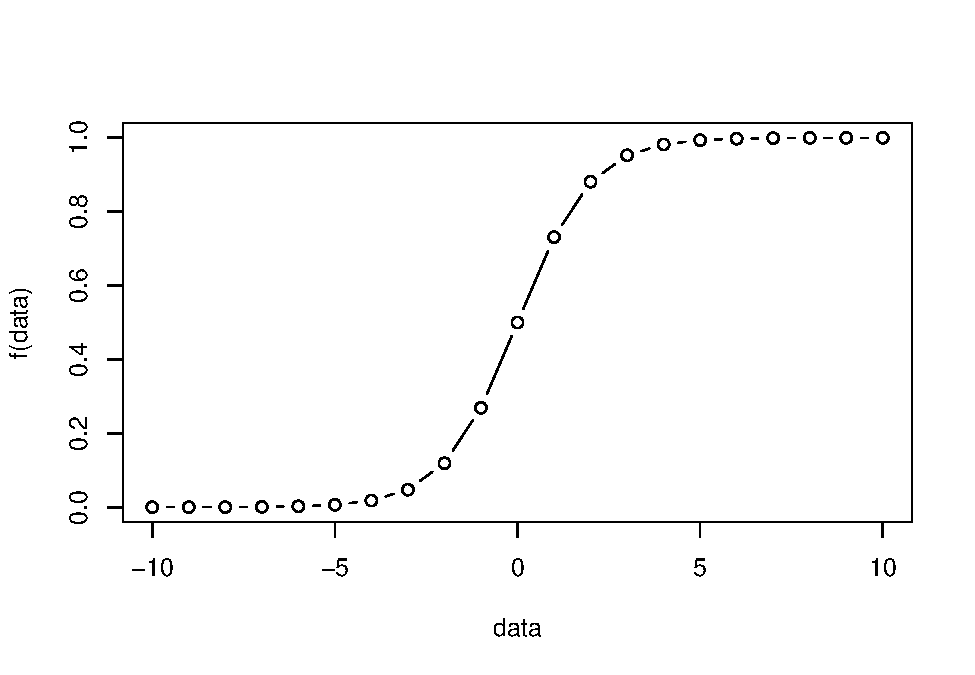
\includegraphics{bookdown-demo_files/figure-latex/unnamed-chunk-1-1.pdf}

We can also write the function into another format as follows:
\[log \frac{p(y=1)}{1-p(y=1)}= \beta_0+\beta_1x_1+...+\beta_nx_n\] Thus,
we know that the regression coeficients of \(\beta_i\) actually change
the ``log-odds'' of the event. Of course, note that the magnitude of
\(\beta_i\) is dependent upon the units of \(x_i\).

The following is an example testing whether that home teams are more
likely to win in NFL games. The results show that the odd of winning is
the same for both home and away teams.

\begin{Shaded}
\begin{Highlighting}[]
\NormalTok{mydata =}\StringTok{ }\KeywordTok{read.csv}\NormalTok{(}\KeywordTok{url}\NormalTok{(}\StringTok{'https://raw.githubusercontent.com/nfl-football-ops/Big-Data-Bowl/master/Data/games.csv'}\NormalTok{))}
\NormalTok{mydata}\OperatorTok{$}\NormalTok{result_new<-}\KeywordTok{ifelse}\NormalTok{(mydata}\OperatorTok{$}\NormalTok{HomeScore}\OperatorTok{>}\NormalTok{mydata}\OperatorTok{$}\NormalTok{VisitorScore,}\DecValTok{1}\NormalTok{,}\DecValTok{0}\NormalTok{)}
\KeywordTok{summary}\NormalTok{(mydata}\OperatorTok{$}\NormalTok{result_new)}
\end{Highlighting}
\end{Shaded}

\begin{verbatim}
##    Min. 1st Qu.  Median    Mean 3rd Qu.    Max. 
##  0.0000  0.0000  0.0000  0.4945  1.0000  1.0000
\end{verbatim}

\begin{Shaded}
\begin{Highlighting}[]
\NormalTok{mylogit1 =}\StringTok{ }\KeywordTok{glm}\NormalTok{(result_new}\OperatorTok{~}\DecValTok{1}\NormalTok{, }\DataTypeTok{family=}\NormalTok{binomial, }\DataTypeTok{data=}\NormalTok{mydata)}
\KeywordTok{summary}\NormalTok{(mylogit1)}
\end{Highlighting}
\end{Shaded}

\begin{verbatim}
## 
## Call:
## glm(formula = result_new ~ 1, family = binomial, data = mydata)
## 
## Deviance Residuals: 
##    Min      1Q  Median      3Q     Max  
## -1.168  -1.168  -1.168   1.187   1.187  
## 
## Coefficients:
##             Estimate Std. Error z value Pr(>|z|)
## (Intercept) -0.02198    0.20967  -0.105    0.917
## 
## (Dispersion parameter for binomial family taken to be 1)
## 
##     Null deviance: 126.14  on 90  degrees of freedom
## Residual deviance: 126.14  on 90  degrees of freedom
## AIC: 128.14
## 
## Number of Fisher Scoring iterations: 3
\end{verbatim}

\section{Probit}\label{probit}

As noted above, logit \(f(x)=log(\frac{p(y=1)}{1-p(y=1)})\) provides the
resulting range of \((0,1)\). Another way to provide the same rage is
through the cdf of normal distribution.The following R code is used to
illusrate this process.

\begin{Shaded}
\begin{Highlighting}[]
\NormalTok{data2<-}\KeywordTok{seq}\NormalTok{(}\OperatorTok{-}\DecValTok{5}\NormalTok{,}\DecValTok{5}\NormalTok{,}\DecValTok{1}\NormalTok{)}
\KeywordTok{plot}\NormalTok{(data2,}\KeywordTok{pnorm}\NormalTok{(data2),}\DataTypeTok{type =} \StringTok{"b"}\NormalTok{)}
\end{Highlighting}
\end{Shaded}

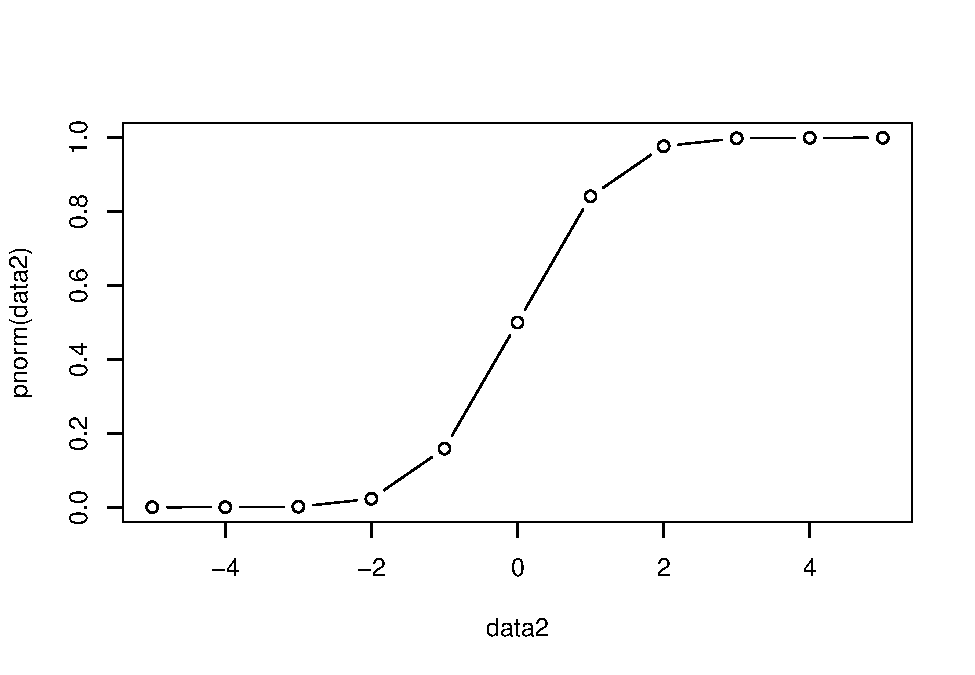
\includegraphics{bookdown-demo_files/figure-latex/unnamed-chunk-3-1.pdf}
Thus, the cdf of normal distribution can be used to indicate the
probability of \(p(y=1)\).

\[\Phi(\beta_0+\beta_1x_1+...+\beta_nx_n )= p(y=1)\]

Similar to logit model, we can also write the inverse function of the
cdf to get the function that can be from \(-\infty\) to \(+\infty\).

\[\beta_0+\beta_1x_1+...+\beta_nx_n =\Phi^{-1}(p(y=1))\]

Thus, for example, if \(X\beta\) = -2, based on
\(\Phi(\beta_0+\beta_1x_1+...+\beta_nx_n )= p(y=1)\) we can get that the
\(p(y=1)=0.023\).

In contrast, if \(X\beta\) = 3, the \(p(y=1)=0.999\).

\begin{Shaded}
\begin{Highlighting}[]
\KeywordTok{pnorm}\NormalTok{(}\OperatorTok{-}\DecValTok{2}\NormalTok{)}
\end{Highlighting}
\end{Shaded}

\begin{verbatim}
## [1] 0.02275013
\end{verbatim}

\begin{Shaded}
\begin{Highlighting}[]
\KeywordTok{pnorm}\NormalTok{(}\DecValTok{3}\NormalTok{)}
\end{Highlighting}
\end{Shaded}

\begin{verbatim}
## [1] 0.9986501
\end{verbatim}

Let's assume that there is a latent variable called \(Y^*\) such that

\[Y^*=X\beta+\epsilon, \epsilon \sim N(0,\sigma^2)\] You could think of
\(Y^*\) as a kind of ``proxy'' between \(X\beta+\epsilon\) and the
observed \(Y (1 or 0)\). Thus, we can get the following. Note that, it
does not have to be zero, and can be any constant.

\[
Y^*=\begin{cases} 0 \;\;\: if \;  y_i^* \leq 0 \\ 1 \;\;\: if \;  y_i^* > 0 \end{cases}
\]

Thus,

\[y_i^* > 0 \Rightarrow \beta^{'}X_i + \epsilon_i >0 \Rightarrow \epsilon_i > -\beta^{'}X_i\]

Thus, we can write it as follows. Note that
\(\frac{ \epsilon_i}{\sigma} \sim N(0,1)\)

\[p(y=1|x_i)= p(y_i^* >0|x_i)=p(\epsilon_i > -\beta^{'}X_i)= p(\frac{ \epsilon_i}{\sigma}>\frac{-\beta^{'}X_i}{\sigma})=\Phi(\frac{\beta^{'}X_i}{\sigma}) \]
We thus can get:

\[p(y=0|x_i)=1-\Phi(\frac{\beta^{'}X_i}{\sigma})\]

For \(p(y=1|x_i)=\Phi(\frac{\beta^{'}X_i}{\sigma})\), we can not really
estimate both \(\beta\) and \(\sigma\) as they are in a ratio. We can
assume \(\sigma =1\), then \(\epsilon \sim N(0,1)\). We know \(y_i\) and
\(x_i\) since we observe them. Thus, we can write it as follows.

\[p(y=1|x_i)=\Phi(\beta^{'}X_i)\]

\chapter{MLE}\label{intro}

\section{Basic idea of MLE}\label{basic-idea-of-mle}

Suppose that we flip a coin, \(y_i=0\) for tails and \(y_i=1\) for
heads. If we get \(p\) heads from \(n\) trials, we can get the
proportion of heads is \(p/n\), which is the sample mean. If we do not
do any further calculation, this is our best guess.

Suppose that the true proablity is \(\rho\), then we can get:

\[
\mathbf{L}(y_i)=\begin{cases} \rho \;\;\:   y_i = 1 \\ 1-\rho \;\;\:  y_i = 0 \end{cases}
\] Thus, we can also write it as follows.
\[\mathbf{L}(y_i) = \rho^{y_i}(1-\rho)^{1-y_i}\]

Thus, we can get:

\[\prod \mathbf{L}(y_i|\rho)=\rho^{\sum y_i}(1-\rho)^{\sum(1-y_i)}\]
Further, we can get a log-transformed format.

\[log (\prod \mathbf{L}(y_i|\rho))=\sum y_i log \rho + \sum(1-y_i) log(1-\rho)\]

To maximize the log-function above, we can calculate the derivative with
respect to \(\rho\).
\[\frac{\partial log (\prod \mathbf{L}(y_i|\rho)) }{\partial \rho}=\sum y_i \frac{1}{\rho}-\sum(1-y_i) \frac{1}{1-\rho}\]
Set the derivative to zero and solve for \(\rho\), we can get

\[\sum y_i \frac{1}{\rho}-\sum(1-y_i) \frac{1}{1-\rho}=0\]
\[\Rightarrow (1-\rho)\sum y_i - \rho \sum(1-y_i) =0\]
\[\Rightarrow \sum y_i-\rho\sum y_i - n\rho +\rho\sum y_i =0\]
\[\Rightarrow \sum y_i - n\rho  =0\]
\[\Rightarrow \rho  = \frac{\sum y_i}{n}=\frac{p}{n}\] Thus, we can see
that the \(\rho\) maximizing the likelihood function is equal to the
sample mean.

\section{Coin flip example, probit, and
logit}\label{coin-flip-example-probit-and-logit}

In the example above, we are not really trying to estimate a lot of
regression coefficients. What we are doing actually is to calculate the
sample mean, or intercept in the regresion sense. What does it mean?
Let's use some data to explain it.

Suppose that we flip a coin 20 times and observe 8 heads. We can use the
R's glm function to esimate the \(\rho\). If the result is consistent
with what we did above, we should observe that the \(cdf\) of the
esimate of \(\beta_0\) (i.e., intercept) should be equal to
\(8/20=0.4\).

\begin{Shaded}
\begin{Highlighting}[]
\NormalTok{coins<-}\KeywordTok{c}\NormalTok{(}\KeywordTok{rep}\NormalTok{(}\DecValTok{1}\NormalTok{,}\DataTypeTok{times=}\DecValTok{8}\NormalTok{),}\KeywordTok{rep}\NormalTok{(}\DecValTok{0}\NormalTok{,}\DataTypeTok{times=}\DecValTok{12}\NormalTok{))}
\KeywordTok{table}\NormalTok{(coins)}
\end{Highlighting}
\end{Shaded}

\begin{verbatim}
## coins
##  0  1 
## 12  8
\end{verbatim}

\begin{Shaded}
\begin{Highlighting}[]
\NormalTok{coins<-}\KeywordTok{as.data.frame}\NormalTok{(coins)}
\end{Highlighting}
\end{Shaded}

\subsection{Probit}\label{probit-1}

\begin{Shaded}
\begin{Highlighting}[]
\NormalTok{probitresults <-}\StringTok{ }\KeywordTok{glm}\NormalTok{(coins }\OperatorTok{~}\StringTok{ }\DecValTok{1}\NormalTok{, }\DataTypeTok{family =} \KeywordTok{binomial}\NormalTok{(}\DataTypeTok{link =} \StringTok{"probit"}\NormalTok{), }\DataTypeTok{data =}\NormalTok{ coins)}
\NormalTok{probitresults}
\end{Highlighting}
\end{Shaded}

\begin{verbatim}
## 
## Call:  glm(formula = coins ~ 1, family = binomial(link = "probit"), 
##     data = coins)
## 
## Coefficients:
## (Intercept)  
##     -0.2533  
## 
## Degrees of Freedom: 19 Total (i.e. Null);  19 Residual
## Null Deviance:       26.92 
## Residual Deviance: 26.92     AIC: 28.92
\end{verbatim}

\begin{Shaded}
\begin{Highlighting}[]
\KeywordTok{pnorm}\NormalTok{(probitresults}\OperatorTok{$}\NormalTok{coefficients)}
\end{Highlighting}
\end{Shaded}

\begin{verbatim}
## (Intercept) 
##         0.4
\end{verbatim}

As we can see the intercept is \(-0.2533\), and thus
\(\Phi(-0.2533471)=0.4\)

\subsection{Logit}\label{logit-1}

We can also use logit link to calculate the intercept as well. Recall
that

\[p(y=1)=\frac{1}{1+e^{-(\beta_0+\beta_1x_1+...+\beta_nx_n)}}=\frac{e^{\beta_0+\beta_1x_1+...+\beta_nx_n}}{1+e^{\beta_0+\beta_1x_1+...+\beta_nx_n}}\]
Thus,

\[p(y=1)=\frac{e^{\beta_0}}{1+e^{\beta_0}}\]

\begin{Shaded}
\begin{Highlighting}[]
\NormalTok{logitresults <-}\StringTok{ }\KeywordTok{glm}\NormalTok{(coins }\OperatorTok{~}\StringTok{ }\DecValTok{1}\NormalTok{, }\DataTypeTok{family =} \KeywordTok{binomial}\NormalTok{(}\DataTypeTok{link =} \StringTok{"logit"}\NormalTok{), }\DataTypeTok{data =}\NormalTok{ coins)}
\NormalTok{logitresults}\OperatorTok{$}\NormalTok{coefficients}
\end{Highlighting}
\end{Shaded}

\begin{verbatim}
## (Intercept) 
##  -0.4054651
\end{verbatim}

\begin{Shaded}
\begin{Highlighting}[]
\KeywordTok{exp}\NormalTok{(logitresults}\OperatorTok{$}\NormalTok{coefficients)}\OperatorTok{/}\NormalTok{(}\DecValTok{1}\OperatorTok{+}\KeywordTok{exp}\NormalTok{(logitresults}\OperatorTok{$}\NormalTok{coefficients))}
\end{Highlighting}
\end{Shaded}

\begin{verbatim}
## (Intercept) 
##         0.4
\end{verbatim}

Note that, the defaul link for the binomial in the glm function in
logit.

\section{Further on logit}\label{further-on-logit}

The probablity of \(y=1\) is as follows:

\[p=p(y=1)=\frac{1}{1+e^{-(\beta_0+\beta_1x_1+...+\beta_nx_n)}}=\frac{e^{\beta_0+\beta_1x_1+...+\beta_nx_n}}{1+e^{\beta_0+\beta_1x_1+...+\beta_nx_n}}\]

Thus, the likelihood function is as follows:

\[L=\prod p^{y_i}(1-p)^{1-y_i}=\prod (\frac{1}{1+e^{-(\beta_0+\beta_1x_1+...+\beta_nx_n)}})^{y_i}(\frac{1}{1+e^{\beta_0+\beta_1x_1+...+\beta_nx_n}})^{1-y_i}\]

\[=\prod (1+e^{-(\beta_0+\beta_1x_1+...+\beta_nx_n)})^{-y_i}(1+e^{\beta_0+\beta_1x_1+...+\beta_nx_n})^{-(1-y_i)}\]

Thus, the log-likelihood is as follows:
\[logL=\sum (-y_i \cdot log(1+e^{-(\beta_0+\beta_1x_1+...+\beta_nx_n)})-(1-y_i)\cdot log(1+e^{\beta_0+\beta_1x_1+...+\beta_nx_n}))\]

Typically, optimisers minimize a function, so we use negative
log-likelihood as minimising that is equivalent to maximising the
log-likelihood or the likelihood itself.

\begin{Shaded}
\begin{Highlighting}[]
\CommentTok{#Source of R code: https://www.r-bloggers.com/logistic-regression/}

\NormalTok{mle.logreg =}\StringTok{ }\ControlFlowTok{function}\NormalTok{(fmla, data)}
\NormalTok{\{}
  \CommentTok{# Define the negative log likelihood function}
\NormalTok{  logl <-}\StringTok{ }\ControlFlowTok{function}\NormalTok{(theta,x,y)\{}
\NormalTok{    y <-}\StringTok{ }\NormalTok{y}
\NormalTok{    x <-}\StringTok{ }\KeywordTok{as.matrix}\NormalTok{(x)}
\NormalTok{    beta <-}\StringTok{ }\NormalTok{theta[}\DecValTok{1}\OperatorTok{:}\KeywordTok{ncol}\NormalTok{(x)]}
    
    \CommentTok{# Use the log-likelihood of the Bernouilli distribution, where p is}
    \CommentTok{# defined as the logistic transformation of a linear combination}
    \CommentTok{# of predictors, according to logit(p)=(x%*%beta)}
\NormalTok{    loglik <-}\StringTok{ }\KeywordTok{sum}\NormalTok{(}\OperatorTok{-}\NormalTok{y}\OperatorTok{*}\KeywordTok{log}\NormalTok{(}\DecValTok{1} \OperatorTok{+}\StringTok{ }\KeywordTok{exp}\NormalTok{(}\OperatorTok{-}\NormalTok{(x}\OperatorTok\NormalTok{beta))) }\OperatorTok{-}\StringTok{ }\NormalTok{(}\DecValTok{1}\OperatorTok{-}\NormalTok{y)}\OperatorTok{*}\KeywordTok{log}\NormalTok{(}\DecValTok{1} \OperatorTok{+}\StringTok{ }\KeywordTok{exp}\NormalTok{(x}\OperatorTok\NormalTok{beta)))}
    \KeywordTok{return}\NormalTok{(}\OperatorTok{-}\NormalTok{loglik)}
\NormalTok{  \}}
  
  \CommentTok{# Prepare the data}
\NormalTok{  outcome =}\StringTok{ }\KeywordTok{rownames}\NormalTok{(}\KeywordTok{attr}\NormalTok{(}\KeywordTok{terms}\NormalTok{(fmla),}\StringTok{"factors"}\NormalTok{))[}\DecValTok{1}\NormalTok{]}
\NormalTok{  dfrTmp =}\StringTok{ }\KeywordTok{model.frame}\NormalTok{(data)}
\NormalTok{  x =}\StringTok{ }\KeywordTok{as.matrix}\NormalTok{(}\KeywordTok{model.matrix}\NormalTok{(fmla, }\DataTypeTok{data=}\NormalTok{dfrTmp))}
\NormalTok{  y =}\StringTok{ }\KeywordTok{as.numeric}\NormalTok{(}\KeywordTok{as.matrix}\NormalTok{(data[,}\KeywordTok{match}\NormalTok{(outcome,}\KeywordTok{colnames}\NormalTok{(data))]))}
  
  \CommentTok{# Define initial values for the parameters}
\NormalTok{  theta.start =}\StringTok{ }\KeywordTok{rep}\NormalTok{(}\DecValTok{0}\NormalTok{,(}\KeywordTok{dim}\NormalTok{(x)[}\DecValTok{2}\NormalTok{]))}
  \KeywordTok{names}\NormalTok{(theta.start) =}\StringTok{ }\KeywordTok{colnames}\NormalTok{(x)}
  
  \CommentTok{# Calculate the maximum likelihood}
\NormalTok{  mle =}\StringTok{ }\KeywordTok{optim}\NormalTok{(theta.start,logl,}\DataTypeTok{x=}\NormalTok{x,}\DataTypeTok{y=}\NormalTok{y, }\DataTypeTok{method =} \StringTok{'BFGS'}\NormalTok{, }\DataTypeTok{hessian=}\NormalTok{T)}
\NormalTok{  out =}\StringTok{ }\KeywordTok{list}\NormalTok{(}\DataTypeTok{beta=}\NormalTok{mle}\OperatorTok{$}\NormalTok{par,}\DataTypeTok{vcov=}\KeywordTok{solve}\NormalTok{(mle}\OperatorTok{$}\NormalTok{hessian),}\DataTypeTok{ll=}\DecValTok{2}\OperatorTok{*}\NormalTok{mle}\OperatorTok{$}\NormalTok{value)}
\NormalTok{\}}
\end{Highlighting}
\end{Shaded}

\begin{Shaded}
\begin{Highlighting}[]
\NormalTok{mydata =}\StringTok{ }\KeywordTok{read.csv}\NormalTok{(}\KeywordTok{url}\NormalTok{(}\StringTok{'https://stats.idre.ucla.edu/stat/data/binary.csv'}\NormalTok{))}
\NormalTok{mylogit1 =}\StringTok{ }\KeywordTok{glm}\NormalTok{(admit}\OperatorTok{~}\NormalTok{gre}\OperatorTok{+}\NormalTok{gpa}\OperatorTok{+}\KeywordTok{as.factor}\NormalTok{(rank), }\DataTypeTok{family=}\NormalTok{binomial, }\DataTypeTok{data=}\NormalTok{mydata)}

\NormalTok{mydata}\OperatorTok{$}\NormalTok{rank =}\StringTok{ }\KeywordTok{factor}\NormalTok{(mydata}\OperatorTok{$}\NormalTok{rank) }\CommentTok{#Treat rank as a categorical variable}
\NormalTok{fmla =}\StringTok{ }\KeywordTok{as.formula}\NormalTok{(}\StringTok{"admit~gre+gpa+rank"}\NormalTok{) }\CommentTok{#Create model formula}
\NormalTok{mylogit2 =}\StringTok{ }\KeywordTok{mle.logreg}\NormalTok{(fmla, mydata) }\CommentTok{#Estimate coefficients}


 \KeywordTok{print}\NormalTok{(}\KeywordTok{cbind}\NormalTok{(}\KeywordTok{coef}\NormalTok{(mylogit1), mylogit2}\OperatorTok{$}\NormalTok{beta))}
\end{Highlighting}
\end{Shaded}

\begin{verbatim}
##                          [,1]         [,2]
## (Intercept)      -3.989979073 -3.772676422
## gre               0.002264426  0.001375522
## gpa               0.804037549  0.898201239
## as.factor(rank)2 -0.675442928 -0.675543009
## as.factor(rank)3 -1.340203916 -1.356554831
## as.factor(rank)4 -1.551463677 -1.563396035
\end{verbatim}

\section{Fisher information}\label{fisher-information}

\url{https://people.missouristate.edu/songfengzheng/Teaching/MTH541/Lecture\%20notes/Fisher_info.pdf}

\section{References}\label{references}

\url{http://www.columbia.edu/~so33/SusDev/Lecture_9.pdf}

\chapter{Linear Mixed Models}\label{linear-mixed-models}

The following is a shortened version of Jonathan Rosenblatt's LMM
tutorial. \url{http://www.john-ros.com/Rcourse/lme.html}.

In addition, another reference is from Douglas Bates's R package
document.
\url{https://cran.r-project.org/web/packages/lme4/vignettes/lmer.pdf?fbclid=IwAR1nmmRP9A0BrhKdgBibNjM5acR_spTpXV8QlQGdmTWyQz3ZtV3LYn6kCbQ}

Assume that \(y\) is a function of \(x\) and \(u\), where \(x\) is the
fixed effect and \(u\) is the random effect. Thus, we can get,

\[y|x, u = x'\beta+z'u+\epsilon\]

For random effect, one example can be that you want to test the
treatment effect, and sample 8 observations from 4 groups. You measure
before and after the treatment. In this case, \(x\) represents the
treatment effect, whereas \(z\) represents the group effect (i.e.,
random effect). Note that, in this case, it reminds the paired t-test.
Remember in SPSS, why do we do paired t-test? Typically, it is the case
when we measure a subject (or, participant) twice. In this case, we can
consider each participant as an unit of random effect (rather than as
group in the last example.)

\section{Calculate mean}\label{calculate-mean}

The following code generates 4 numbers (\(N(0,10)\)) for 4 groups. Then,
replicate it within each group.That is, in the end, there are 8
observations.

Note that, in the following code, there are no ``independent
variables''. Both the linear model and mixed model are actually just
trying to calculate the mean. Note that
lmer(y\textasciitilde{}1+1\textbar{}groups) and
lmer(y\textasciitilde{}1\textbar{}groups) will generate the same
results.

\begin{Shaded}
\begin{Highlighting}[]
\KeywordTok{set.seed}\NormalTok{(}\DecValTok{123}\NormalTok{)}
\NormalTok{n.groups <-}\StringTok{ }\DecValTok{4} \CommentTok{# number of groups}
\NormalTok{n.repeats <-}\StringTok{ }\DecValTok{2} \CommentTok{# samples per group}
\CommentTok{#Generating index for observations belong to the same group}
\NormalTok{groups <-}\StringTok{ }\KeywordTok{as.factor}\NormalTok{(}\KeywordTok{rep}\NormalTok{(}\DecValTok{1}\OperatorTok{:}\NormalTok{n.groups, }\DataTypeTok{each=}\NormalTok{n.repeats))}
\NormalTok{n <-}\StringTok{ }\KeywordTok{length}\NormalTok{(groups)}
\CommentTok{#Generating 4 random numbers, assuming normal distribution}
\NormalTok{z0 <-}\StringTok{ }\KeywordTok{rnorm}\NormalTok{(n.groups, }\DecValTok{0}\NormalTok{, }\DecValTok{10}\NormalTok{) }
\NormalTok{z <-}\StringTok{ }\NormalTok{z0[}\KeywordTok{as.numeric}\NormalTok{(groups)] }\CommentTok{# generate and inspect random group effects}
\NormalTok{z}
\end{Highlighting}
\end{Shaded}

\begin{verbatim}
## [1] -5.6047565 -5.6047565 -2.3017749 -2.3017749 15.5870831 15.5870831  0.7050839
## [8]  0.7050839
\end{verbatim}

\begin{Shaded}
\begin{Highlighting}[]
\NormalTok{epsilon <-}\StringTok{ }\KeywordTok{rnorm}\NormalTok{(n,}\DecValTok{0}\NormalTok{,}\DecValTok{1}\NormalTok{) }\CommentTok{# generate measurement error}
\NormalTok{beta0 <-}\StringTok{ }\DecValTok{2} \CommentTok{# this is the actual parameter of interest! The global mean.}
\NormalTok{y <-}\StringTok{ }\NormalTok{beta0 }\OperatorTok{+}\StringTok{ }\NormalTok{z }\OperatorTok{+}\StringTok{ }\NormalTok{epsilon }\CommentTok{# sample from an LMM}

\CommentTok{# fit a linear model assuming independence}
\CommentTok{# i.e., assume that there is no "group things".}
\NormalTok{lm.}\DecValTok{5}\NormalTok{ <-}\StringTok{ }\KeywordTok{lm}\NormalTok{(y}\OperatorTok{~}\DecValTok{1}\NormalTok{)}

\CommentTok{# fit a mixed-model that deals with the group dependence}
\CommentTok{#install.packages("lme4")}
\KeywordTok{library}\NormalTok{(lme4)}
\NormalTok{lme.}\FloatTok{5.}\NormalTok{a <-}\StringTok{ }\KeywordTok{lmer}\NormalTok{(y}\OperatorTok{~}\DecValTok{1}\OperatorTok{+}\DecValTok{1}\OperatorTok{|}\NormalTok{groups) }
\NormalTok{lme.}\FloatTok{5.}\NormalTok{b <-}\StringTok{ }\KeywordTok{lmer}\NormalTok{(y}\OperatorTok{~}\DecValTok{1}\OperatorTok{|}\NormalTok{groups) }
\NormalTok{lm.}\DecValTok{5}
\end{Highlighting}
\end{Shaded}

\begin{verbatim}
## 
## Call:
## lm(formula = y ~ 1)
## 
## Coefficients:
## (Intercept)  
##       4.283
\end{verbatim}

\begin{Shaded}
\begin{Highlighting}[]
\NormalTok{lme.}\FloatTok{5.}\NormalTok{a }
\end{Highlighting}
\end{Shaded}

\begin{verbatim}
## Linear mixed model fit by REML ['lmerMod']
## Formula: y ~ 1 + 1 | groups
## REML criterion at convergence: 36.1666
## Random effects:
##  Groups   Name        Std.Dev.
##  groups   (Intercept) 8.8521  
##  Residual             0.8873  
## Number of obs: 8, groups:  groups, 4
## Fixed Effects:
## (Intercept)  
##       4.283
\end{verbatim}

\begin{Shaded}
\begin{Highlighting}[]
\NormalTok{lme.}\FloatTok{5.}\NormalTok{b }
\end{Highlighting}
\end{Shaded}

\begin{verbatim}
## Linear mixed model fit by REML ['lmerMod']
## Formula: y ~ 1 | groups
## REML criterion at convergence: 36.1666
## Random effects:
##  Groups   Name        Std.Dev.
##  groups   (Intercept) 8.8521  
##  Residual             0.8873  
## Number of obs: 8, groups:  groups, 4
## Fixed Effects:
## (Intercept)  
##       4.283
\end{verbatim}

\section{Test the treatment effect}\label{test-the-treatment-effect}

As we can see that, LLM and paired t-test generate the same t-value.

\begin{Shaded}
\begin{Highlighting}[]
\NormalTok{times<-}\KeywordTok{rep}\NormalTok{(}\KeywordTok{c}\NormalTok{(}\DecValTok{1}\NormalTok{,}\DecValTok{2}\NormalTok{),}\DecValTok{4}\NormalTok{) }\CommentTok{# first time and second time}
\NormalTok{times}
\end{Highlighting}
\end{Shaded}

\begin{verbatim}
## [1] 1 2 1 2 1 2 1 2
\end{verbatim}

\begin{Shaded}
\begin{Highlighting}[]
\NormalTok{data_combined<-}\KeywordTok{cbind}\NormalTok{(y,groups,times)}
\NormalTok{data_combined}
\end{Highlighting}
\end{Shaded}

\begin{verbatim}
##               y groups times
## [1,] -3.4754687      1     1
## [2,] -1.8896915      1     2
## [3,]  0.1591413      2     1
## [4,] -1.5668361      2     2
## [5,] 16.9002303      3     1
## [6,] 17.1414212      3     2
## [7,]  3.9291657      4     1
## [8,]  3.0648977      4     2
\end{verbatim}

\begin{Shaded}
\begin{Highlighting}[]
\NormalTok{lme_diff_times<-}\StringTok{ }\KeywordTok{lmer}\NormalTok{(y}\OperatorTok{~}\NormalTok{times}\OperatorTok{+}\NormalTok{(}\DecValTok{1}\OperatorTok{|}\NormalTok{groups)) }


\NormalTok{t_results<-}\KeywordTok{t.test}\NormalTok{(y}\OperatorTok{~}\NormalTok{times, }\DataTypeTok{paired=}\OtherTok{TRUE}\NormalTok{)}

\NormalTok{lme_diff_times}
\end{Highlighting}
\end{Shaded}

\begin{verbatim}
## Linear mixed model fit by REML ['lmerMod']
## Formula: y ~ times + (1 | groups)
## REML criterion at convergence: 35.0539
## Random effects:
##  Groups   Name        Std.Dev.
##  groups   (Intercept) 8.845   
##  Residual             1.013   
## Number of obs: 8, groups:  groups, 4
## Fixed Effects:
## (Intercept)        times  
##      4.5691      -0.1908
\end{verbatim}

\begin{Shaded}
\begin{Highlighting}[]
\KeywordTok{print}\NormalTok{(}\StringTok{"The following results are from paired t-test"}\NormalTok{)}
\end{Highlighting}
\end{Shaded}

\begin{verbatim}
## [1] "The following results are from paired t-test"
\end{verbatim}

\begin{Shaded}
\begin{Highlighting}[]
\NormalTok{t_results}\OperatorTok{$}\NormalTok{statistic}
\end{Highlighting}
\end{Shaded}

\begin{verbatim}
##         t 
## 0.2664793
\end{verbatim}

\section{Another example}\label{another-example}

\begin{Shaded}
\begin{Highlighting}[]
\KeywordTok{data}\NormalTok{(Dyestuff, }\DataTypeTok{package=}\StringTok{'lme4'}\NormalTok{)}
\KeywordTok{attach}\NormalTok{(Dyestuff)}
\end{Highlighting}
\end{Shaded}

\begin{verbatim}
## The following objects are masked from Dyestuff (pos = 6):
## 
##     Batch, Yield
\end{verbatim}

\begin{Shaded}
\begin{Highlighting}[]
\NormalTok{Dyestuff}
\end{Highlighting}
\end{Shaded}

\begin{verbatim}
##    Batch Yield
## 1      A  1545
## 2      A  1440
## 3      A  1440
## 4      A  1520
## 5      A  1580
## 6      B  1540
## 7      B  1555
## 8      B  1490
## 9      B  1560
## 10     B  1495
## 11     C  1595
## 12     C  1550
## 13     C  1605
## 14     C  1510
## 15     C  1560
## 16     D  1445
## 17     D  1440
## 18     D  1595
## 19     D  1465
## 20     D  1545
## 21     E  1595
## 22     E  1630
## 23     E  1515
## 24     E  1635
## 25     E  1625
## 26     F  1520
## 27     F  1455
## 28     F  1450
## 29     F  1480
## 30     F  1445
\end{verbatim}

\begin{Shaded}
\begin{Highlighting}[]
\NormalTok{lme_batch<-}\StringTok{ }\KeywordTok{lmer}\NormalTok{( Yield }\OperatorTok{~}\StringTok{ }\DecValTok{1} \OperatorTok{+}\StringTok{ }\NormalTok{(}\DecValTok{1}\OperatorTok{|}\NormalTok{Batch)  , Dyestuff )}
\KeywordTok{summary}\NormalTok{(lme_batch)}
\end{Highlighting}
\end{Shaded}

\begin{verbatim}
## Linear mixed model fit by REML ['lmerMod']
## Formula: Yield ~ 1 + (1 | Batch)
##    Data: Dyestuff
## 
## REML criterion at convergence: 319.7
## 
## Scaled residuals: 
##     Min      1Q  Median      3Q     Max 
## -1.4117 -0.7634  0.1418  0.7792  1.8296 
## 
## Random effects:
##  Groups   Name        Variance Std.Dev.
##  Batch    (Intercept) 1764     42.00   
##  Residual             2451     49.51   
## Number of obs: 30, groups:  Batch, 6
## 
## Fixed effects:
##             Estimate Std. Error t value
## (Intercept)  1527.50      19.38    78.8
\end{verbatim}

\section{Full LMM model}\label{full-lmm-model}

In the following, I used the data from the package of lme4. For Days +
(1 \textbar{} Subject), it only has random intercept; in contrast, Days
+ ( Days\textbar{} Subject ) has both random intercept and random slope
for Days. Note that, random effects do not generate specific slopes for
each level of Days, but rather just a variance of all the slopes.

Therefore, we can see that ``Days + ( Days\textbar{} Subject )'' and
``Days + ( 1+Days\textbar{} Subject )'' generate the same results. For
more discussion, you can refer to the following link:
\url{https://www.jaredknowles.com/journal/2013/11/25/getting-started-with-mixed-effect-models-in-r}

\begin{Shaded}
\begin{Highlighting}[]
\KeywordTok{data}\NormalTok{(sleepstudy, }\DataTypeTok{package=}\StringTok{'lme4'}\NormalTok{)}
\KeywordTok{attach}\NormalTok{(sleepstudy)}
\end{Highlighting}
\end{Shaded}

\begin{verbatim}
## The following objects are masked from sleepstudy (pos = 6):
## 
##     Days, Reaction, Subject
\end{verbatim}

\begin{Shaded}
\begin{Highlighting}[]
\NormalTok{fm1 <-}\StringTok{ }\KeywordTok{lmer}\NormalTok{(Reaction }\OperatorTok{~}\StringTok{ }\NormalTok{Days }\OperatorTok{+}\StringTok{ }\NormalTok{(}\DecValTok{1} \OperatorTok{|}\StringTok{ }\NormalTok{Subject), sleepstudy)}
\KeywordTok{summary}\NormalTok{(fm1)}
\end{Highlighting}
\end{Shaded}

\begin{verbatim}
## Linear mixed model fit by REML ['lmerMod']
## Formula: Reaction ~ Days + (1 | Subject)
##    Data: sleepstudy
## 
## REML criterion at convergence: 1786.5
## 
## Scaled residuals: 
##     Min      1Q  Median      3Q     Max 
## -3.2257 -0.5529  0.0109  0.5188  4.2506 
## 
## Random effects:
##  Groups   Name        Variance Std.Dev.
##  Subject  (Intercept) 1378.2   37.12   
##  Residual              960.5   30.99   
## Number of obs: 180, groups:  Subject, 18
## 
## Fixed effects:
##             Estimate Std. Error t value
## (Intercept) 251.4051     9.7467   25.79
## Days         10.4673     0.8042   13.02
## 
## Correlation of Fixed Effects:
##      (Intr)
## Days -0.371
\end{verbatim}

\begin{Shaded}
\begin{Highlighting}[]
\NormalTok{fm2<-}\KeywordTok{lmer}\NormalTok{ ( Reaction }\OperatorTok{~}\StringTok{ }\NormalTok{Days }\OperatorTok{+}\StringTok{ }\NormalTok{( Days}\OperatorTok{|}\StringTok{ }\NormalTok{Subject ) , }\DataTypeTok{data=}\NormalTok{ sleepstudy )}
\KeywordTok{summary}\NormalTok{(fm2)}
\end{Highlighting}
\end{Shaded}

\begin{verbatim}
## Linear mixed model fit by REML ['lmerMod']
## Formula: Reaction ~ Days + (Days | Subject)
##    Data: sleepstudy
## 
## REML criterion at convergence: 1743.6
## 
## Scaled residuals: 
##     Min      1Q  Median      3Q     Max 
## -3.9536 -0.4634  0.0231  0.4633  5.1793 
## 
## Random effects:
##  Groups   Name        Variance Std.Dev. Corr
##  Subject  (Intercept) 611.90   24.737       
##           Days         35.08    5.923   0.07
##  Residual             654.94   25.592       
## Number of obs: 180, groups:  Subject, 18
## 
## Fixed effects:
##             Estimate Std. Error t value
## (Intercept)  251.405      6.824  36.843
## Days          10.467      1.546   6.771
## 
## Correlation of Fixed Effects:
##      (Intr)
## Days -0.138
\end{verbatim}

\begin{Shaded}
\begin{Highlighting}[]
\NormalTok{fm3<-}\KeywordTok{lmer}\NormalTok{ ( Reaction }\OperatorTok{~}\StringTok{ }\NormalTok{Days }\OperatorTok{+}\StringTok{ }\NormalTok{(}\DecValTok{1}\OperatorTok{+}\NormalTok{Days}\OperatorTok{|}\StringTok{ }\NormalTok{Subject ) , }\DataTypeTok{data=}\NormalTok{ sleepstudy )}
\KeywordTok{summary}\NormalTok{(fm3)}
\end{Highlighting}
\end{Shaded}

\begin{verbatim}
## Linear mixed model fit by REML ['lmerMod']
## Formula: Reaction ~ Days + (1 + Days | Subject)
##    Data: sleepstudy
## 
## REML criterion at convergence: 1743.6
## 
## Scaled residuals: 
##     Min      1Q  Median      3Q     Max 
## -3.9536 -0.4634  0.0231  0.4633  5.1793 
## 
## Random effects:
##  Groups   Name        Variance Std.Dev. Corr
##  Subject  (Intercept) 611.90   24.737       
##           Days         35.08    5.923   0.07
##  Residual             654.94   25.592       
## Number of obs: 180, groups:  Subject, 18
## 
## Fixed effects:
##             Estimate Std. Error t value
## (Intercept)  251.405      6.824  36.843
## Days          10.467      1.546   6.771
## 
## Correlation of Fixed Effects:
##      (Intr)
## Days -0.138
\end{verbatim}

\section{Serial correlations in time and
space}\label{serial-correlations-in-time-and-space}

The hierarchical model of \(y|x, u = x'\beta+z'u+\epsilon\) can work
well for correlations within blocks, but not for correlations in time as
the correlations decay in time. The following uses nlme package to
calculate time serial data.

\begin{Shaded}
\begin{Highlighting}[]
\KeywordTok{library}\NormalTok{(nlme)}
\KeywordTok{head}\NormalTok{(nlme}\OperatorTok{::}\NormalTok{Ovary,}\DataTypeTok{n=}\DecValTok{50}\NormalTok{)}
\end{Highlighting}
\end{Shaded}

\begin{verbatim}
## Grouped Data: follicles ~ Time | Mare
##    Mare        Time follicles
## 1     1 -0.13636360        20
## 2     1 -0.09090910        15
## 3     1 -0.04545455        19
## 4     1  0.00000000        16
## 5     1  0.04545455        13
## 6     1  0.09090910        10
## 7     1  0.13636360        12
## 8     1  0.18181820        14
## 9     1  0.22727270        13
## 10    1  0.27272730        20
## 11    1  0.31818180        22
## 12    1  0.36363640        15
## 13    1  0.40909090        18
## 14    1  0.45454550        17
## 15    1  0.50000000        14
## 16    1  0.54545450        18
## 17    1  0.59090910        14
## 18    1  0.63636360        16
## 19    1  0.68181820        17
## 20    1  0.72727270        18
## 21    1  0.77272730        18
## 22    1  0.81818180        17
## 23    1  0.86363640        14
## 24    1  0.90909090        12
## 25    1  0.95454550        12
## 26    1  1.00000000        14
## 27    1  1.04545500        10
## 28    1  1.09090900        11
## 29    1  1.13636400        16
## 30    2 -0.15000000         6
## 31    2 -0.10000000         6
## 32    2 -0.05000000         8
## 33    2  0.00000000         7
## 34    2  0.05000000        16
## 35    2  0.10000000        10
## 36    2  0.15000000        13
## 37    2  0.20000000         9
## 38    2  0.25000000         7
## 39    2  0.30000000         6
## 40    2  0.35000000         8
## 41    2  0.40000000         8
## 42    2  0.45000000         6
## 43    2  0.50000000         8
## 44    2  0.55000000         7
## 45    2  0.60000000         9
## 46    2  0.65000000         6
## 47    2  0.70000000         4
## 48    2  0.75000000         5
## 49    2  0.80000000         8
## 50    2  0.85000000        11
\end{verbatim}

\begin{Shaded}
\begin{Highlighting}[]
\NormalTok{fm1Ovar.lme <-}\StringTok{ }\NormalTok{nlme}\OperatorTok{::}\KeywordTok{lme}\NormalTok{(}\DataTypeTok{fixed=}\NormalTok{follicles }\OperatorTok{~}\StringTok{ }\KeywordTok{sin}\NormalTok{(}\DecValTok{2}\OperatorTok{*}\NormalTok{pi}\OperatorTok{*}\NormalTok{Time) }\OperatorTok{+}\StringTok{ }\KeywordTok{cos}\NormalTok{(}\DecValTok{2}\OperatorTok{*}\NormalTok{pi}\OperatorTok{*}\NormalTok{Time), }
                   \DataTypeTok{data =}\NormalTok{ Ovary, }
                   \DataTypeTok{random =} \KeywordTok{pdDiag}\NormalTok{(}\OperatorTok{~}\KeywordTok{sin}\NormalTok{(}\DecValTok{2}\OperatorTok{*}\NormalTok{pi}\OperatorTok{*}\NormalTok{Time)), }
                   \DataTypeTok{correlation=}\KeywordTok{corAR1}\NormalTok{() )}
\KeywordTok{summary}\NormalTok{(fm1Ovar.lme)}
\end{Highlighting}
\end{Shaded}

\begin{verbatim}
## Linear mixed-effects model fit by REML
##  Data: Ovary 
##        AIC     BIC   logLik
##   1563.448 1589.49 -774.724
## 
## Random effects:
##  Formula: ~sin(2 * pi * Time) | Mare
##  Structure: Diagonal
##         (Intercept) sin(2 * pi * Time) Residual
## StdDev:    2.858385           1.257977 3.507053
## 
## Correlation Structure: AR(1)
##  Formula: ~1 | Mare 
##  Parameter estimate(s):
##       Phi 
## 0.5721866 
## Fixed effects: follicles ~ sin(2 * pi * Time) + cos(2 * pi * Time) 
##                        Value Std.Error  DF   t-value p-value
## (Intercept)        12.188089 0.9436602 295 12.915760  0.0000
## sin(2 * pi * Time) -2.985297 0.6055968 295 -4.929513  0.0000
## cos(2 * pi * Time) -0.877762 0.4777821 295 -1.837159  0.0672
##  Correlation: 
##                    (Intr) s(*p*T
## sin(2 * pi * Time)  0.000       
## cos(2 * pi * Time) -0.123  0.000
## 
## Standardized Within-Group Residuals:
##         Min          Q1         Med          Q3         Max 
## -2.34910093 -0.58969626 -0.04577893  0.52931186  3.37167486 
## 
## Number of Observations: 308
## Number of Groups: 11
\end{verbatim}

\chapter{Basic Concepts}\label{basic-concepts}

\section{Score}\label{score}

The score is the gradient (the vector of partial derivatives) of
\(log L(\theta)\), with respect to an m-dimensional parameter vector
\(\theta\).

\[S(\theta) = \frac{\partial\ell}{\partial \theta}\]

Such differentiation will generate a \(m\times 1\) row vector, which
indicates the sensitivity of the likelihood.

Quote from Steffen Lauritzen's slides: ``Generally the solution to this
equation must be calculated by iterative methods. One of the most common
methods is the Newton--Raphson method and this is based on successive
approximations to the solution, using Taylor's theorem to approximate
the equation.''

For instance, using logit link, we can get the first derivative of log
likelihood logistic regression as follows. We can not really find
\(\beta\) easily to make the equation to be 0.

\[\frac{\partial \ell} {\partial \beta} = \sum_{i=1}^{n}x_i^T[y_i-\frac{e^{\beta^Tx_i}}{1+e^{\beta^Tx_i}}]\]

\section{Canonical link function}\label{canonical-link-function}

References: Steffen Lauritzen's slides:
\url{http://www.stats.ox.ac.uk/~steffen/teaching/bs2HT9/scoring.pdf}

\chapter{Generalized Linear Mixed
Models}\label{generalized-linear-mixed-models}

\section{Computing techniques}\label{computing-techniques}

Since GLMM can use EM algorithm in its maximum likelihood calculation
(see McCulloch, 1994), it is practically useful to rehearse EM and other
computing techniques.

\subsection{Monte carlo approximation}\label{monte-carlo-approximation}

Example: calculate the integral of \(p(z>2)\) when \(z \sim N(0,1)\). To
use Monte Carlo approximation, we can have an indicator function, which
will determine whether the sample from \(N(0,1)\) will be included into
the calculation of the integral.

\begin{Shaded}
\begin{Highlighting}[]
\NormalTok{Nsim=}\DecValTok{10}\OperatorTok{^}\DecValTok{4}

\NormalTok{indicator=}\ControlFlowTok{function}\NormalTok{(x)\{}
\NormalTok{y=}\KeywordTok{ifelse}\NormalTok{((x}\OperatorTok{>}\DecValTok{2}\NormalTok{),}\DecValTok{1}\NormalTok{,}\DecValTok{0}\NormalTok{)}
\KeywordTok{return}\NormalTok{(y)\}}

\NormalTok{newdata<-}\KeywordTok{rnorm}\NormalTok{(Nsim, }\DecValTok{0}\NormalTok{,}\DecValTok{1}\NormalTok{ )}

\NormalTok{mc=}\KeywordTok{c}\NormalTok{(); v=}\KeywordTok{c}\NormalTok{(); upper=}\KeywordTok{c}\NormalTok{(); lower=}\KeywordTok{c}\NormalTok{()}

\ControlFlowTok{for}\NormalTok{ (j }\ControlFlowTok{in} \DecValTok{1}\OperatorTok{:}\NormalTok{Nsim)}
\NormalTok{\{}
\NormalTok{mc[j]=}\KeywordTok{mean}\NormalTok{(}\KeywordTok{indicator}\NormalTok{(newdata[}\DecValTok{1}\OperatorTok{:}\NormalTok{j]))}
\NormalTok{v[j]=(j}\OperatorTok{^}\NormalTok{\{}\OperatorTok{-}\DecValTok{1}\NormalTok{\})}\OperatorTok{*}\KeywordTok{var}\NormalTok{(}\KeywordTok{indicator}\NormalTok{(newdata[}\DecValTok{1}\OperatorTok{:}\NormalTok{j]))}
\NormalTok{upper[j]=mc[j]}\OperatorTok{+}\FloatTok{1.96}\OperatorTok{*}\KeywordTok{sqrt}\NormalTok{(v[j])}
\NormalTok{lower[j]=mc[j]}\OperatorTok{-}\FloatTok{1.96}\OperatorTok{*}\KeywordTok{sqrt}\NormalTok{(v[j])}
\NormalTok{\}}

\KeywordTok{library}\NormalTok{(ggplot2)}
\NormalTok{values=}\KeywordTok{c}\NormalTok{(mc,upper,lower)}
\NormalTok{type=}\KeywordTok{c}\NormalTok{(}\KeywordTok{rep}\NormalTok{(}\StringTok{"mc"}\NormalTok{,Nsim),}\KeywordTok{rep}\NormalTok{(}\StringTok{"upper"}\NormalTok{,Nsim),}\KeywordTok{rep}\NormalTok{(}\StringTok{"lower"}\NormalTok{,Nsim))}
\NormalTok{iter=}\KeywordTok{rep}\NormalTok{(}\KeywordTok{seq}\NormalTok{(}\DecValTok{1}\OperatorTok{:}\NormalTok{Nsim),}\DecValTok{3}\NormalTok{)}
\NormalTok{data=}\KeywordTok{data.frame}\NormalTok{(}\DataTypeTok{val=}\NormalTok{values, }\DataTypeTok{tp=}\NormalTok{type, }\DataTypeTok{itr=}\NormalTok{iter)}
\NormalTok{Rcode<-}\KeywordTok{ggplot}\NormalTok{(data,}\KeywordTok{aes}\NormalTok{(itr,val,}\DataTypeTok{col=}\NormalTok{tp))}\OperatorTok{+}\KeywordTok{geom_line}\NormalTok{(}\DataTypeTok{size=}\FloatTok{0.5}\NormalTok{)}
\NormalTok{Rcode}\OperatorTok{+}\KeywordTok{geom_hline}\NormalTok{(}\DataTypeTok{yintercept=}\DecValTok{1}\OperatorTok{-}\KeywordTok{pnorm}\NormalTok{(}\DecValTok{2}\NormalTok{),}\DataTypeTok{color=}\StringTok{"green"}\NormalTok{,}\DataTypeTok{size=}\FloatTok{0.5}\NormalTok{)}
\end{Highlighting}
\end{Shaded}

\begin{verbatim}
## Warning: Removed 2 rows containing missing values (geom_path).
\end{verbatim}

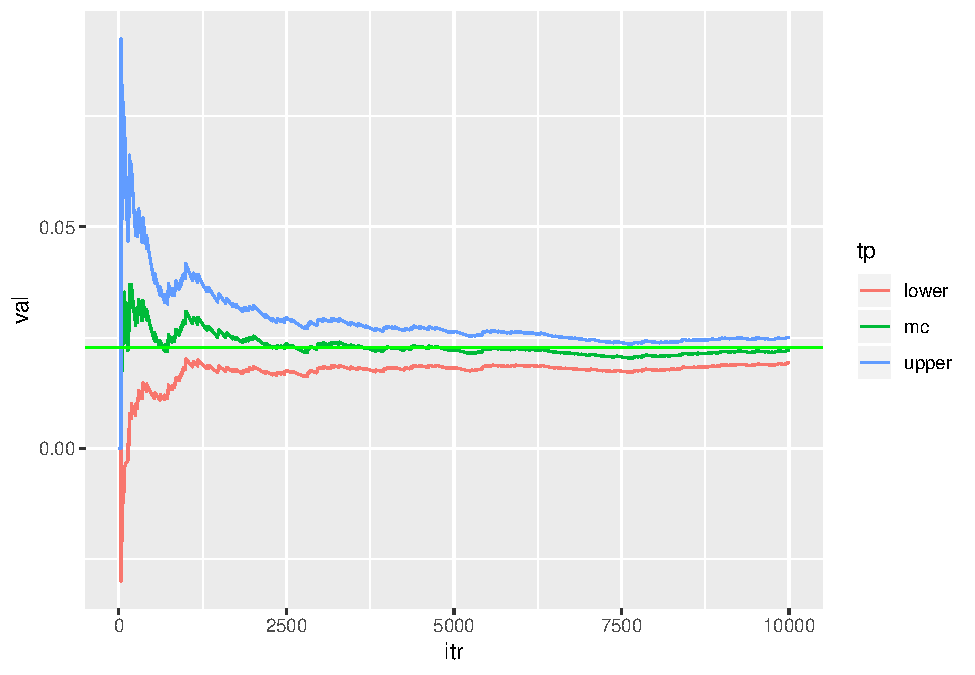
\includegraphics{bookdown-demo_files/figure-latex/unnamed-chunk-16-1.pdf}

\subsection{Importance sampling}\label{importance-sampling}

Importance sampling has samples generated from a different distribution
than the distribution of interest. Specifically, assume that we want to
calculate the expected value of \(h(x)\), and \(x \sim f(x)\).

\[E(h(x))=\int h(x) f(x) dx = \int h(x) \frac{f(x)}{g(x)} g(x) dx \] We
can sample \(x_i\) from \(g(x)\) and then calculate the mean of
\(h(x_i) \frac{f(x_i)}{g(x_i)}\).

Using the same explane above, we can use a shifted exponential
distribution to help calculate the intergral for normal distribution.
Specifically,

\[\int_2^{\infty} \frac{1}{2 \pi} e^{-\frac{1}{2}x^2}dx = \int_2^{\infty} \frac{\frac{1}{2 \pi} e^{-\frac{1}{2}x^2}}{e^{-(x-2)}} e^{-(x-2)}dx \]
The idea is that, we can generate \(x_i\) from exponential distribution
of \(e^{-(x-2)}\), and then insert them into the targeted ``expected
(value) function'' of
\(\frac{\frac{1}{2 \pi} e^{-\frac{1}{2}x^2}}{e^{-(x-2)}}\). Thus, as you
can see, importance sampling is based on the law of large numbers (i.e.,
If the same experiment or study is repeated independently a large number
of times, the average of the results of the trials must be close to the
expected value). We can use it to calculate integral based on link of
the definition of expected value.

\begin{Shaded}
\begin{Highlighting}[]
\NormalTok{Nsim=}\DecValTok{10}\OperatorTok{^}\DecValTok{4}
\NormalTok{normal_density=}\ControlFlowTok{function}\NormalTok{(x)}
\NormalTok{\{y=(}\DecValTok{1}\OperatorTok{/}\KeywordTok{sqrt}\NormalTok{(}\DecValTok{2}\OperatorTok{*}\NormalTok{pi))}\OperatorTok{*}\KeywordTok{exp}\NormalTok{(}\OperatorTok{-}\FloatTok{0.5}\OperatorTok{*}\NormalTok{(x}\OperatorTok{^}\DecValTok{2}\NormalTok{))}
\KeywordTok{return}\NormalTok{(y)\}}
\NormalTok{x=}\DecValTok{2}\OperatorTok{-}\KeywordTok{log}\NormalTok{(}\KeywordTok{runif}\NormalTok{(Nsim))}
\NormalTok{ImpS=}\KeywordTok{c}\NormalTok{(); v=}\KeywordTok{c}\NormalTok{(); upper=}\KeywordTok{c}\NormalTok{(); lower=}\KeywordTok{c}\NormalTok{()}
\ControlFlowTok{for}\NormalTok{ (j }\ControlFlowTok{in} \DecValTok{1}\OperatorTok{:}\NormalTok{Nsim)}
\NormalTok{\{}
\NormalTok{ImpS[j]=}\KeywordTok{mean}\NormalTok{(}\KeywordTok{normal_density}\NormalTok{(x[}\DecValTok{1}\OperatorTok{:}\NormalTok{j])}\OperatorTok{/}\KeywordTok{exp}\NormalTok{(}\OperatorTok{-}\NormalTok{(x[}\DecValTok{1}\OperatorTok{:}\NormalTok{j]}\OperatorTok{-}\DecValTok{2}\NormalTok{)))}
\NormalTok{v[j]=(j}\OperatorTok{^}\NormalTok{\{}\OperatorTok{-}\DecValTok{1}\NormalTok{\})}\OperatorTok{*}\KeywordTok{var}\NormalTok{(}\KeywordTok{normal_density}\NormalTok{(x[}\DecValTok{1}\OperatorTok{:}\NormalTok{j])}\OperatorTok{/}\KeywordTok{exp}\NormalTok{(}\OperatorTok{-}\NormalTok{(x[}\DecValTok{1}\OperatorTok{:}\NormalTok{j]}\OperatorTok{-}\DecValTok{2}\NormalTok{)))}
\NormalTok{upper[j]=ImpS[j]}\OperatorTok{+}\FloatTok{1.96}\OperatorTok{*}\KeywordTok{sqrt}\NormalTok{(v[j])}
\NormalTok{lower[j]=ImpS[j]}\OperatorTok{-}\FloatTok{1.96}\OperatorTok{*}\KeywordTok{sqrt}\NormalTok{(v[j])}
\NormalTok{\}}

\KeywordTok{library}\NormalTok{(ggplot2)}
\NormalTok{values=}\KeywordTok{c}\NormalTok{(ImpS,upper,lower)}
\NormalTok{type=}\KeywordTok{c}\NormalTok{(}\KeywordTok{rep}\NormalTok{(}\StringTok{"mc"}\NormalTok{,Nsim),}\KeywordTok{rep}\NormalTok{(}\StringTok{"upper"}\NormalTok{,Nsim),}\KeywordTok{rep}\NormalTok{(}\StringTok{"lower"}\NormalTok{,Nsim))}
\NormalTok{iter=}\KeywordTok{rep}\NormalTok{(}\KeywordTok{seq}\NormalTok{(}\DecValTok{1}\OperatorTok{:}\NormalTok{Nsim),}\DecValTok{3}\NormalTok{)}
\NormalTok{data=}\KeywordTok{data.frame}\NormalTok{(}\DataTypeTok{val=}\NormalTok{values, }\DataTypeTok{tp=}\NormalTok{type, }\DataTypeTok{itr=}\NormalTok{iter)}
\KeywordTok{ggplot}\NormalTok{(data,}\KeywordTok{aes}\NormalTok{(itr,val,}\DataTypeTok{col=}\NormalTok{tp))}\OperatorTok{+}\KeywordTok{geom_line}\NormalTok{(}\DataTypeTok{size=}\FloatTok{0.5}\NormalTok{)}\OperatorTok{+}
\KeywordTok{geom_hline}\NormalTok{(}\DataTypeTok{yintercept=}\DecValTok{1}\OperatorTok{-}\KeywordTok{pnorm}\NormalTok{(}\DecValTok{2}\NormalTok{),}\DataTypeTok{color=}\StringTok{"green"}\NormalTok{,}\DataTypeTok{size=}\FloatTok{0.5}\NormalTok{)}
\end{Highlighting}
\end{Shaded}

\begin{verbatim}
## Warning: Removed 2 rows containing missing values (geom_path).
\end{verbatim}

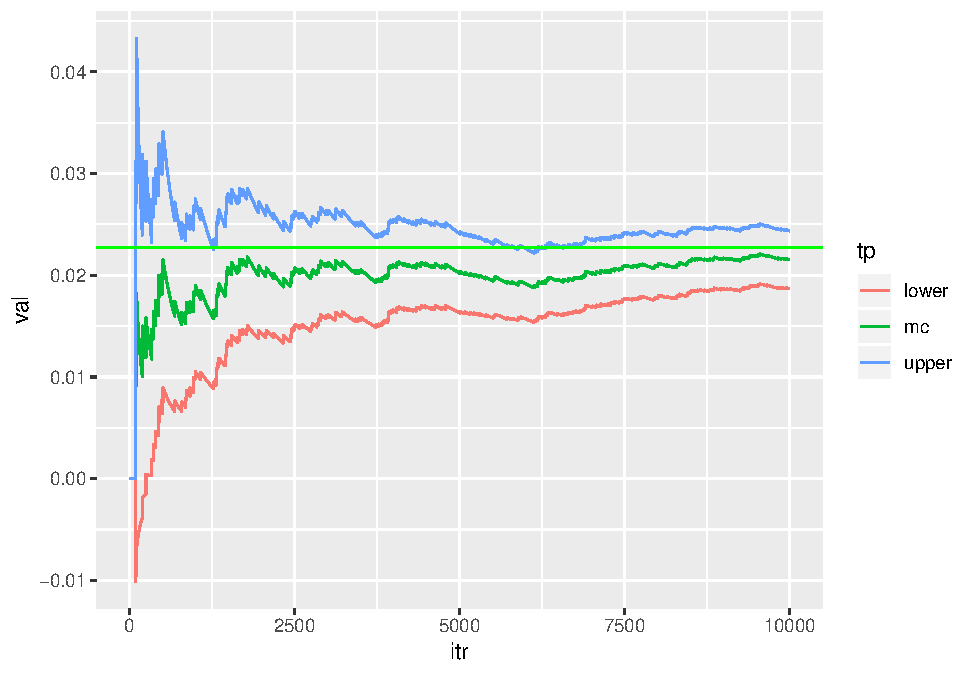
\includegraphics{bookdown-demo_files/figure-latex/unnamed-chunk-17-1.pdf}

\subsection{Newton Raphson algorithm}\label{newton-raphson-algorithm}

For nonlinear functions, it is sometimes difficult to calculate MLEs.
Newton Raphson algorithm is an iterative procedure to calculate MLEs.

The basic idea of Newton Raphson is to find a approximate function that
can be easily maximized analytically. We need some theoretical
background from Taylor's Theorem.

If \(f\) has \(k+1\) times differentiable on an open interval \(I\). For
any \(x\) and \(x+h\) in \(I\), there is a point of \(w\) between \(x\)
and \(x+h\) where we can get the following:

\[f(x+h)=f(x)+f^{'}h+\frac{1}{2}f^{''}h^2+...+\frac{1}{k!}f^{[k]}(x)h^k+\frac{1}{(k+1)!}f^{[k+1]}(w)h^{k+1}\]
If \(h\) goes to be close to \(0\), the higher order terms will go to
\(0\) as well. Thus, we can get:

\[f(x+h) \approx f(x)+f^{'}(x)h \] This is the first order Taylor
approximation of \(f\) at \(x\). In a similar vein, we also have the
second order Taylor approximation of \(f\) at \(x\) as follows.

\[f(x+h)=f(x)+f^{'}h+\frac{1}{2}f^{''}h^2\] For the first order, we can
rewrite it as follows.

\[f(x+h) \approx f(x)+f^{'}(x)h = a+bh\] where,

\[ a = f(x), b=f^{'}(x)\] Similarly,

\[f(x+h)\approx f(x)+f^{'}(x)h+\frac{1}{2}f^{''}(x)h^2=a+bh+\frac{1}{2}ch^2\]
We can calculate the derivative with respect to \(h\), we can get:

\[f^{'}(x+h) \approx b+ch\] We can then set it to zero, and get:

\[0=b+c \hat{h}\] Thus, we can get,

\[\hat{h} = -\frac{b}{c}=-\frac{f^{'}(x)}{f^{''}(x)}\] Thus, we can get
that the following can maximize \(f\) at \(x\):

\[x+\hat{h}=x-\frac{f^{'}(x)}{f^{''}(x)}\] Thus, the basic idea of
Newton Raphson algorithm is as follows. - set a tolerance (typically a
very small number) - Check if \(|f^{'}(x)|< the tolerance\). If not,
\(i \leftarrow i+1; x_i\leftarrow x_{i-1}-\frac{f^{'}(x_{i-1})}{f^{''}(x_{i-1})}\)

Practice:

\begin{enumerate}
\def\labelenumi{(\arabic{enumi})}
\tightlist
\item
  Solve the \(x^3-5=0\)
\end{enumerate}

Note that, this is obviously not a maximization problem. In contrast, it
involves a function with zero. As we can see, we can think it as the
first order of Taylor approximation. That is, \(f^{'}(x)=x^3-5=0\). As
we can see the following plot, it converts very quickly. {[}I will
revisit this part later to double check whether such narrative is
correct. But, the code is correct, for sure.{]}

\begin{Shaded}
\begin{Highlighting}[]
\NormalTok{f_firstorder=}\ControlFlowTok{function}\NormalTok{(x)\{x}\OperatorTok{^}\DecValTok{3}\OperatorTok{-}\DecValTok{5}\NormalTok{\}}
\NormalTok{f_secondorder=}\ControlFlowTok{function}\NormalTok{(x)\{}\DecValTok{3}\OperatorTok{*}\NormalTok{x\}}
\NormalTok{x_old=}\DecValTok{1}\NormalTok{;tolerance=}\FloatTok{1e-3}
\NormalTok{max_its=}\DecValTok{2000}\NormalTok{;iteration=}\DecValTok{1}\NormalTok{;difference=}\DecValTok{2}
\NormalTok{c_iteration<-}\KeywordTok{c}\NormalTok{() ## to collect numbers generated in the iteration process }
\ControlFlowTok{while}\NormalTok{(difference}\OperatorTok{>}\NormalTok{tolerance }\OperatorTok{&}\StringTok{ }\NormalTok{iteration}\OperatorTok{<}\NormalTok{max_its)\{}
\NormalTok{  x_updated=x_old}\OperatorTok{-}\NormalTok{(}\KeywordTok{f_firstorder}\NormalTok{(x_old)}\OperatorTok{/}\KeywordTok{f_secondorder}\NormalTok{(x_old))}
\NormalTok{  difference=}\KeywordTok{abs}\NormalTok{(x_updated}\OperatorTok{-}\NormalTok{x_old);}
\NormalTok{  iteration=iteration}\OperatorTok{+}\DecValTok{1}\NormalTok{;}
\NormalTok{  x_old=x_updated}
\NormalTok{  c_iteration<-}\KeywordTok{c}\NormalTok{(c_iteration,x_updated)\}}

\KeywordTok{plot}\NormalTok{(c_iteration,}\DataTypeTok{type=}\StringTok{"b"}\NormalTok{)}
\end{Highlighting}
\end{Shaded}

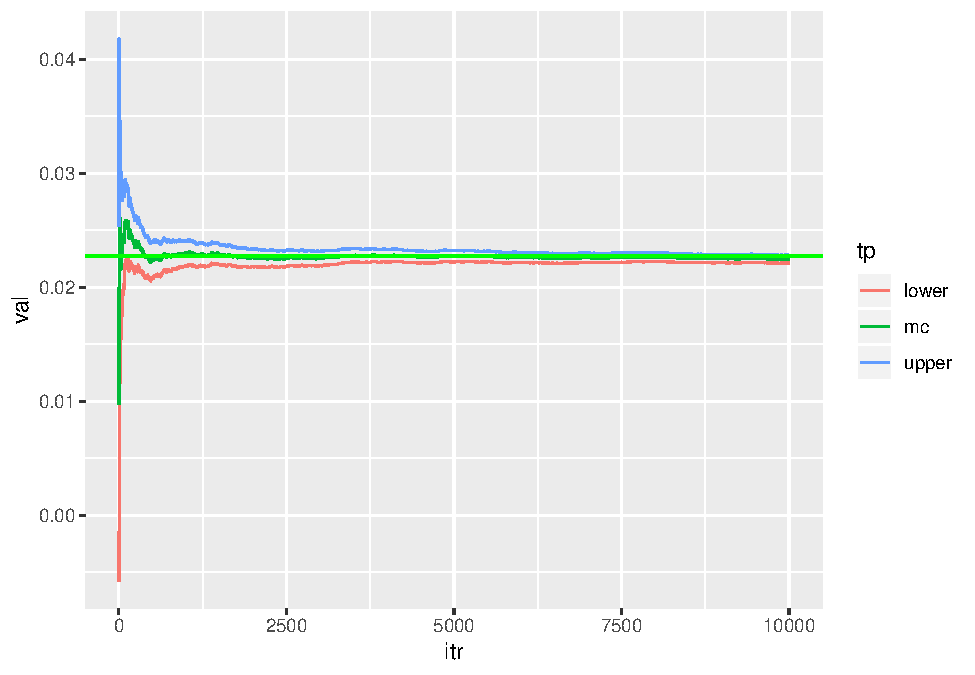
\includegraphics{bookdown-demo_files/figure-latex/unnamed-chunk-18-1.pdf}

\begin{enumerate}
\def\labelenumi{\arabic{enumi}.}
\setcounter{enumi}{1}
\tightlist
\item
  Use Newton Raphson to calculate the logistic regression
\end{enumerate}

Suppose we have \(n\) observation, and \(m\) variables.

\[\begin{bmatrix}
x_{11} & x_{12} & x_{13} & ... & x_{1m}\\
x_{21} & x_{22} & x_{23} & ... & x_{2m} \\
...\\
x_{n1} & x_{n2} & x_{n3} & ... & x_{nm}
\end{bmatrix}\]

Typically, we add a vector of \(1\) being used to estimate the constant.

\[\begin{bmatrix}
1 & x_{11} & x_{12} & x_{13} & ... & x_{1m}\\
1 & x_{21} & x_{22} & x_{23} & ... & x_{2m} \\
...\\
1 & x_{n1} & x_{n2} & x_{n3} & ... & x_{nm}
\end{bmatrix}\]

And, we have observe a vector of \(n\) \(y_i\) as well, which is a
binary variable:

\[Y = \begin{bmatrix}1 \\
0 \\
1 \\
0 \\
0 \\
0 \\
...\\
1 \\
\end{bmatrix}\]

Using the content from the MLE chapter, we can get:

\[\mathbf{L}=\prod_{i=1}^{n} p_i^{ y_i}(1-p_i)^{(1-y_i)}\]

Further, we can get a log-transformed format.

\[log (\mathbf{L})=\sum_{i=1}^{n}[y_i log (p_i) + (1-y_i) log(1-p_i)]\]
Given that
\(p_i=\frac{e^{\beta_0+\beta_1x_1+...+\beta_nx_n}}{1+e^{\beta_0+\beta_1x_1+...+\beta_nx_n}}=\frac{e^{\beta^Tx}}{1+e^{\beta^Tx}}\),
we can rewrite it as follows:

\[log (\mathbf{L})=\ell=\sum_{i=1}^{n}[y_i log (\frac{e^{\beta^Tx_i}}{1+e^{\beta^Tx_i}}) + (1-y_i) log(1-\frac{e^{\beta^Tx_i}}{1+e^{\beta^Tx_i}})]\]
Before doing the derivative, we set.
\[\frac{e^{\beta^Tx_i}}{1+e^{\beta^Tx_i}} = p(\beta ^T x_i)\]

\[log (\mathbf{L})=\ell=\sum_{i=1}^{n}[y_i log (p(\beta ^T x_i)) + (1-y_i) log(1-p(\beta ^T x_i))]\]

Note that,
\(\frac{\partial p(\beta ^T x_i)}{\partial (\beta ^T x_i)} = p(\beta ^T x_i)(1-p(\beta ^T x_i))\).
We will use it later.

\[\begin{aligned}
\frac{\partial \ell} {\partial \beta} &= \sum_{i=1}^{n} [y_i \frac{1}{p(\beta ^T x_i)} \frac{\partial p(\beta ^T x_i)}{\partial (\beta ^T x_i)}\frac{\partial (\beta ^T x_i)}{\partial \beta}+(1-y_i) \frac{1}{1-p(\beta ^T x_i)}(-1)\frac{\partial p(\beta ^T x_i)}{\partial (\beta ^T x_i)}\frac{\partial (\beta ^T x_i)}{\partial \beta}] \\
&= \sum_{i=1}^{n} x_i^T[y_i \frac{1}{p(\beta ^T x_i)} p(\beta ^T x_i)(1-p(\beta ^T x_i))+(1-y_i) \frac{1}{1-p(\beta ^T x_i)}(-1)p(\beta ^T x_i)(1-p(\beta ^T x_i))] \\
&= \sum_{i=1}^{n} x_i^T[y_i \frac{1}{p(\beta ^T x_i)} p(\beta ^T x_i)(1-p(\beta ^T x_i))-(1-y_i) \frac{1}{1-p(\beta ^T x_i)}p(\beta ^T x_i)(1-p(\beta ^T x_i))] \\
&= \sum_{i=1}^{n} x_i^T[y_i (1-p(\beta ^T x_i))-(1-y_i) p(\beta ^T x_i)] \\
&=\sum_{i=1}^{n} x_i^T[y_i-y_ip(\beta ^T x_i)-p(\beta ^T x_i)+y_i p(\beta ^T x_i)] \\
&=\sum_{i=1}^{n} x_i^T[y_i-p(\beta ^T x_i)] \\
&= \sum_{i=1}^{n} x_i^T[y_i-\frac{e^{\beta^Tx_i}}{1+e^{\beta^Tx_i}}]
\end{aligned}\]

As noted, the Newton Raphson algorithm needs the second order.

\[\begin{aligned}
Second order &=\frac{\partial \sum_{i=1}^{n} x_i^T[y_i-p(\beta ^T x_i)]}{\partial \beta} \\
&=-\sum_{i=1}^{n} x_i^T\frac{\partial p(\beta ^T x_i) }{\partial \beta}\\
&=-\sum_{i=1}^{n} x_i^T\frac{\partial p(\beta ^T x_i) }{\partial (\beta^Tx_i)} \frac{\partial (\beta^Tx_i)}{\partial \beta}\\
&=-\sum_{i=1}^{n} x_i^T p(\beta ^T x_i)(1-p(\beta ^T x_i))x_i
\end{aligned}\]

The following are the data simulation (3 IVs and 1 DV) and Newton
Raphson analysis.

\begin{Shaded}
\begin{Highlighting}[]
\CommentTok{# Data generation}
\KeywordTok{set.seed}\NormalTok{(}\DecValTok{123}\NormalTok{)}
\NormalTok{n=}\DecValTok{500}
\NormalTok{x1_norm<-}\KeywordTok{rnorm}\NormalTok{(n)}
\NormalTok{x2_norm<-}\KeywordTok{rnorm}\NormalTok{(n,}\DecValTok{3}\NormalTok{,}\DecValTok{4}\NormalTok{)}
\NormalTok{x3_norm<-}\KeywordTok{rnorm}\NormalTok{(n,}\DecValTok{4}\NormalTok{,}\DecValTok{6}\NormalTok{)}
\NormalTok{x_combined<-}\KeywordTok{cbind}\NormalTok{(}\DecValTok{1}\NormalTok{,x1_norm,x2_norm,x3_norm) }\CommentTok{# dimension: n*4}
\NormalTok{coefficients_new<-}\KeywordTok{c}\NormalTok{(}\DecValTok{1}\NormalTok{,}\DecValTok{2}\NormalTok{,}\DecValTok{3}\NormalTok{,}\DecValTok{4}\NormalTok{)  }\CommentTok{#true regression coefficient}
\NormalTok{inv_logit<-}\ControlFlowTok{function}\NormalTok{(x,b)\{}\KeywordTok{exp}\NormalTok{(x}\OperatorTok\NormalTok{b)}\OperatorTok{/}\NormalTok{(}\DecValTok{1}\OperatorTok{+}\KeywordTok{exp}\NormalTok{(x}\OperatorTok\NormalTok{b))\}}
\NormalTok{prob_generated<-}\KeywordTok{inv_logit}\NormalTok{(x_combined,coefficients_new)}
\NormalTok{y<-}\KeywordTok{c}\NormalTok{()}
\ControlFlowTok{for}\NormalTok{ (i }\ControlFlowTok{in} \DecValTok{1}\OperatorTok{:}\NormalTok{n) \{y[i]<-}\KeywordTok{rbinom}\NormalTok{(}\DecValTok{1}\NormalTok{,}\DecValTok{1}\NormalTok{,prob_generated[i])\}}

\CommentTok{# Newton Raphson}

\CommentTok{#We need to set random starting values.}
\NormalTok{beta_old<-}\KeywordTok{c}\NormalTok{(}\DecValTok{1}\NormalTok{,}\DecValTok{1}\NormalTok{,}\DecValTok{1}\NormalTok{,}\DecValTok{1}\NormalTok{)}
\NormalTok{tolerance=}\FloatTok{1e-3}
\NormalTok{max_its=}\DecValTok{2000}\NormalTok{;iteration=}\DecValTok{1}\NormalTok{;difference=}\DecValTok{2}
\NormalTok{W<-}\KeywordTok{matrix}\NormalTok{(}\DecValTok{0}\NormalTok{,n,n)}

\ControlFlowTok{while}\NormalTok{(difference}\OperatorTok{>}\NormalTok{tolerance }\OperatorTok{&}\StringTok{ }\NormalTok{iteration}\OperatorTok{<}\NormalTok{max_its)}
\NormalTok{  \{}
  \CommentTok{# The first order}
\NormalTok{  f_firstorder<-}\KeywordTok{t}\NormalTok{(x_combined)}\OperatorTok\NormalTok{(y}\OperatorTok{-}\KeywordTok{inv_logit}\NormalTok{(x_combined,beta_old))}
  \CommentTok{# The second order}
  \KeywordTok{diag}\NormalTok{(W) =}\StringTok{ }\KeywordTok{inv_logit}\NormalTok{(x_combined,beta_old)}\OperatorTok{*}\NormalTok{(}\DecValTok{1}\OperatorTok{-}\KeywordTok{inv_logit}\NormalTok{(x_combined,beta_old))}
\NormalTok{  f_secondorder<-}\OperatorTok{-}\KeywordTok{t}\NormalTok{(x_combined)}\OperatorTok\NormalTok{W}\OperatorTok\NormalTok{x_combined}
  \CommentTok{# Calculate the beta_updated}
\NormalTok{  beta_updated=beta_old}\OperatorTok{-}\NormalTok{(}\KeywordTok{solve}\NormalTok{(f_secondorder)}\OperatorTok\NormalTok{f_firstorder)}
\NormalTok{  difference=}\KeywordTok{max}\NormalTok{(}\KeywordTok{abs}\NormalTok{(beta_updated}\OperatorTok{-}\NormalTok{beta_old));}
\NormalTok{  iteration=iteration}\OperatorTok{+}\DecValTok{1}\NormalTok{;}
\NormalTok{  beta_old=beta_updated\}}

\NormalTok{beta_old}
\end{Highlighting}
\end{Shaded}

\begin{verbatim}
##              [,1]
##         0.9590207
## x1_norm 1.7974165
## x2_norm 3.0072303
## x3_norm 3.9578107
\end{verbatim}

\[\frac{\partial \ell} {\partial \beta} = \sum_{i=1}^{n} [y_i \frac{1}{p(\beta ^T x_i)} \frac{\partial p(\beta ^T x_i)}{\partial (\beta ^T x_i)}\frac{\partial (\beta ^T x_i)}{\partial \beta}+(1-y_i) \frac{1}{1-p(\beta ^T x_i)}(-1)\frac{\partial p(\beta ^T x_i)}{\partial (\beta ^T x_i)}\frac{\partial (\beta ^T x_i)}{\partial \beta}] \]
\[=\sum_{i=1}^{n} [y_i \frac{1}{p(\beta ^T x_i)} \phi (\beta ^T x_i)-(1-y_i) \frac{1}{1-p(\beta ^T x_i)}\phi (\beta ^T x_i)]x_i\]

\[\Phi(\beta_0+\beta_1x_1+\beta_2x_2+\beta_3x_3)= p(y=1)\]

\begin{Shaded}
\begin{Highlighting}[]
\CommentTok{# Data generation}
\NormalTok{n=}\DecValTok{500}
\NormalTok{x1_norm<-}\KeywordTok{rnorm}\NormalTok{(n)}
\NormalTok{x2_norm<-}\KeywordTok{rnorm}\NormalTok{(n)}
\NormalTok{x3_norm<-}\KeywordTok{rnorm}\NormalTok{(n)}
\NormalTok{x_combined<-}\KeywordTok{cbind}\NormalTok{(}\DecValTok{1}\NormalTok{,x1_norm,x2_norm,x3_norm)}
\NormalTok{coefficients_new<-}\KeywordTok{c}\NormalTok{(}\DecValTok{2}\NormalTok{,}\DecValTok{2}\NormalTok{,}\DecValTok{3}\NormalTok{,}\DecValTok{3}\NormalTok{)  }\CommentTok{#true regression coefficient}
\NormalTok{inv_norm<-}\ControlFlowTok{function}\NormalTok{(x,b)\{}\KeywordTok{pnorm}\NormalTok{(x}\OperatorTok\NormalTok{b)\}}
\NormalTok{prob_generated<-}\KeywordTok{inv_norm}\NormalTok{(x_combined,coefficients_new)}
\NormalTok{y<-}\KeywordTok{c}\NormalTok{()}
\ControlFlowTok{for}\NormalTok{ (i }\ControlFlowTok{in} \DecValTok{1}\OperatorTok{:}\NormalTok{n) \{y[i]<-}\KeywordTok{rbinom}\NormalTok{(}\DecValTok{1}\NormalTok{,}\DecValTok{1}\NormalTok{,prob_generated[i])\}}

\CommentTok{# Newton Raphson}

\CommentTok{#We need to set random starting values.}
\NormalTok{x_old<-}\KeywordTok{c}\NormalTok{(}\DecValTok{1}\NormalTok{,}\DecValTok{1}\NormalTok{,}\DecValTok{1}\NormalTok{,}\DecValTok{1}\NormalTok{)}
\NormalTok{tolerance=}\FloatTok{1e-3}
\NormalTok{max_its=}\DecValTok{2000}\NormalTok{;iteration=}\DecValTok{1}\NormalTok{;difference=}\DecValTok{2}

\ControlFlowTok{while}\NormalTok{(difference}\OperatorTok{>}\NormalTok{tolerance }\OperatorTok{&}\StringTok{ }\NormalTok{iteration}\OperatorTok{<}\NormalTok{max_its)\{}
\NormalTok{  x_updated=x_old}\OperatorTok{-}\NormalTok{(}\KeywordTok{f_firstorder}\NormalTok{(x_old)}\OperatorTok{/}\KeywordTok{f_secondorder}\NormalTok{(x_old))}
\NormalTok{  difference=}\KeywordTok{abs}\NormalTok{(x_updated}\OperatorTok{-}\NormalTok{x_old);}
\NormalTok{  iteration=iteration}\OperatorTok{+}\DecValTok{1}\NormalTok{;}
\NormalTok{  x_old=x_updated}
\NormalTok{  c_iteration<-}\KeywordTok{c}\NormalTok{(c_iteration,x_updated)\}}

\KeywordTok{plot}\NormalTok{(c_iteration,}\DataTypeTok{type=}\StringTok{"b"}\NormalTok{)}
\end{Highlighting}
\end{Shaded}

Some links related to this topic (canonical link function):
\url{http://www.win-vector.com/blog/2011/09/the-simpler-derivation-of-logistic-regression/}
\url{https://en.wikipedia.org/wiki/Generalized_linear_model\#Link_function}
\url{https://stats.stackexchange.com/questions/40876/what-is-the-difference-between-a-link-function-and-a-canonical-link-function}
\url{https://stats.stackexchange.com/questions/344309/why-using-newtons-method-for-logistic-regression-optimization-is-called-iterati}
\url{https://www.stat.washington.edu/adobra/classes/536/Files/week1/newtonfull.pdf}
\url{https://tomroth.com.au/logistic/}
\url{https://www.stat.cmu.edu/~cshalizi/350/lectures/26/lecture-26.pdf}

\url{http://seankross.com/2019/10/27/R-as-a-First-Programming-Language.html}

\section{Basics of GLMM}\label{basics-of-glmm}

Recall the formula in the probit model:

\[Y^*=X\beta+\epsilon, \epsilon \sim N(0,\sigma^2)=N(0,I)\] Similar to
LMM, binary model with random effect can be written as follows.

\[Y^*=X\beta+ Z u+\epsilon\] where,

\[\epsilon \sim N(0,I)\] \[u \sim N(0, D)\]

We also assume \(\epsilon\) and \(u\) are independent.Thus, we know that
\(D\) represents the virances of the random effects. If we make
\(u =1\), the model becomes the usual probit model. McCulloch (1994)
states that there are a few advantages to use probit, rather than logit
models.

The following is the note from Charle E. McCulloch's ``Maximum
likelihood algorithems for Generalized Linear Mixed Models''

\section{Some References}\label{some-references}

\url{http://www.biostat.umn.edu/~baolin/teaching/linmods/glmm.html}

\url{http://www.biostat.umn.edu/~baolin/teaching/probmods/GLMM_mcmc.html}

\url{https://bbolker.github.io/mixedmodels-misc/glmmFAQ.html}

\chapter{Twitter Example}\label{twitter-example}

The following is part of my course project for Stat 536. It aims to
replicate part of the findings from Barbera (2015) Birds of the Same
Feather Tweet Together: Bayesian Ideal Point Estimation Using Twitter
Data. Political Analysis 23 (1). Note that, the following model is much
simpler than that in the original paper.

\section{Model}\label{model}

Suppose that a Twitter user is presented with a choice between following
or not following another target \(j \in \{ 1, ..., m\}\). Let
\(y_{j}=1\) if the user decides to follow \(j\), and \(y_{j}=0\)
otherwise.

\[y_{j}=\begin{cases} 1 & Following \\ 0 & Not Following \end{cases}\]

\[p(y_{j}=1|\theta) = \frac{exp(- \theta_0|\theta_1 - x_j|^2)}{1+exp(- \theta_0|\theta_1 - x_j|^2)}\]
We additionally know the priors of \(\theta\).

\[\theta_i \sim N(0,10^2) (i = 0, 1)\]

The likelihood function is as follows.

\[L(Y|\theta)=\prod_{j=1}^{m} (\frac{exp(- \theta_0|\theta_1 - x_j|^2)}{1+exp(- \theta_0|\theta_1 - x_j|^2)})^{y_j}(1-\frac{exp(- \theta_0|\theta_1 - x_j|^2)}{1+exp(- \theta_0|\theta_1 - x_j|^2)})^{(1-y_j)}\]
Thus, the posterior is as follows.

\[L(Y|\theta) \cdot N(\theta_0|0,10) \cdot N(\theta_1|0,10)\]
\[\propto \prod_{j=1}^{m} (\frac{exp(- \theta_0|\theta_1 - x_j|^2)}{1+exp(- \theta_0|\theta_1 - x_j|^2)})^{y_j}(1-\frac{exp(- \theta_0|\theta_1 - x_j|^2)}{1+exp(- \theta_0|\theta_1 - x_j|^2)})^{(1-y_j)}\cdot exp(-\frac{1}{2}(\frac{\theta_0}{10})^2)\cdot exp(-\frac{1}{2}(\frac{\theta_1}{10})^2)\]

\section{Simulating Data of Senators on
Twitter}\label{simulating-data-of-senators-on-twitter}

Assume that we have 100 senators, 50 Democrats and 50 Republicans, who
we know their ideology. Assume that Democrats have negative ideology
scores to indicate that they are more liberal, whereas Republicans have
positive scores to indicate that they are more conservative. The
following is data simulation for senators.

\begin{Shaded}
\begin{Highlighting}[]
\CommentTok{# Republicans are more conservative, and they have positive numbers.}
\NormalTok{Republicans<-}\KeywordTok{c}\NormalTok{()}
\NormalTok{Republicans<-}\KeywordTok{rnorm}\NormalTok{(}\DecValTok{50}\NormalTok{,}\DecValTok{1}\NormalTok{,}\FloatTok{0.5}\NormalTok{)}
\NormalTok{No_Republicans<-}\KeywordTok{rep}\NormalTok{(}\DecValTok{1}\OperatorTok{:}\DecValTok{50}\NormalTok{,}\DecValTok{1}\NormalTok{)}
\NormalTok{Part_}\DecValTok{1}\NormalTok{<-}\KeywordTok{cbind}\NormalTok{(No_Republicans,Republicans)}

\CommentTok{# Democrats are more liberal, and they have negative numbers.}
\NormalTok{Democrats<-}\KeywordTok{c}\NormalTok{()}
\NormalTok{Democrats<-}\KeywordTok{rnorm}\NormalTok{(}\DecValTok{50}\NormalTok{,}\OperatorTok{-}\DecValTok{1}\NormalTok{,}\FloatTok{0.5}\NormalTok{)}
\NormalTok{No_Democrats<-}\KeywordTok{rep}\NormalTok{(}\DecValTok{51}\OperatorTok{:}\DecValTok{100}\NormalTok{,}\DecValTok{1}\NormalTok{)}
\NormalTok{Part_}\DecValTok{2}\NormalTok{<-}\KeywordTok{cbind}\NormalTok{(No_Democrats,Democrats)}
\NormalTok{Data_Elites<-}\KeywordTok{rbind}\NormalTok{(Part_}\DecValTok{1}\NormalTok{,Part_}\DecValTok{2}\NormalTok{)}
\NormalTok{Data_Elites<-}\KeywordTok{as.data.frame}\NormalTok{(Data_Elites)}
\KeywordTok{colnames}\NormalTok{(Data_Elites) <-}\StringTok{ }\KeywordTok{c}\NormalTok{(}\StringTok{"Elite_No"}\NormalTok{,}\StringTok{"Elite_ideology"}\NormalTok{)}

\KeywordTok{head}\NormalTok{(Data_Elites)}
\end{Highlighting}
\end{Shaded}

\begin{verbatim}
##   Elite_No Elite_ideology
## 1        1      1.2848895
## 2        2      0.1733722
## 3        3      0.6666728
## 4        4      0.7758829
## 5        5      1.5219457
## 6        6      1.5140870
\end{verbatim}

\section{Simulating Data of Conservative Users on Twitter and Model
Testing}\label{simulating-data-of-conservative-users-on-twitter-and-model-testing}

Assume that we observe one Twitter user, who is more conservative. To
simulate Twitter following data for this user, I assign this user to
follow more Republican senators. Thus, if the Metropolis Hastings
algorithm works as intended, we would expect to see a positive estimated
value for their ideology. Importantly, as we can see in the histogram
below, the estimated value indeed is positive, providing preliminary
evidence for the statistical model and the algorithm. In addition, for
the acceptance rate, we can see that the constant has a lower number
than ideology, since we only accept a constant when it is positive.

\begin{Shaded}
\begin{Highlighting}[]
\CommentTok{#This user approximately follows 45 Republican Senators and 10 Democrat Senators. }
\NormalTok{Data_user<-}\KeywordTok{as.data.frame}\NormalTok{(}\KeywordTok{matrix}\NormalTok{(}\KeywordTok{c}\NormalTok{(}\KeywordTok{ifelse}\NormalTok{(}\KeywordTok{runif}\NormalTok{(}\DecValTok{50}\NormalTok{)}\OperatorTok{<}\NormalTok{.}\DecValTok{1}\NormalTok{,}\DecValTok{0}\NormalTok{,}\DecValTok{1}\NormalTok{),}\KeywordTok{ifelse}\NormalTok{(}\KeywordTok{runif}\NormalTok{(}\DecValTok{50}\NormalTok{)}\OperatorTok{<}\NormalTok{.}\DecValTok{8}\NormalTok{,}\DecValTok{0}\NormalTok{,}\DecValTok{1}\NormalTok{))), }\DecValTok{100}\NormalTok{, }\DecValTok{1}\NormalTok{)}
\KeywordTok{colnames}\NormalTok{(Data_user)<-}\KeywordTok{c}\NormalTok{(}\StringTok{"R_User"}\NormalTok{)}
\NormalTok{Data_combined<-}\KeywordTok{cbind}\NormalTok{(Data_Elites,Data_user)}

\NormalTok{X_data<-Data_combined}\OperatorTok{$}\NormalTok{Elite_ideology}
\NormalTok{Y_data<-Data_combined}\OperatorTok{$}\NormalTok{R_User}

\NormalTok{fit_C<-}\KeywordTok{Bayes_logit}\NormalTok{(Y_data,X_data)}
\NormalTok{fit_C}\OperatorTok{$}\NormalTok{acceptance_rate}
\end{Highlighting}
\end{Shaded}

\begin{verbatim}
## [1] 0.1590795 0.4817409
\end{verbatim}

\begin{Shaded}
\begin{Highlighting}[]
\KeywordTok{plot}\NormalTok{(fit_C}\OperatorTok{$}\NormalTok{theta[,}\DecValTok{1}\NormalTok{],}\DataTypeTok{main=}\StringTok{"Constant (Conservative Users)"}\NormalTok{,}
     \DataTypeTok{xlab=}\StringTok{"Iteration Process"}\NormalTok{,}\DataTypeTok{ylab=}\StringTok{"Estimated Scores"}\NormalTok{,}\DataTypeTok{type=}\StringTok{"l"}\NormalTok{)}
\end{Highlighting}
\end{Shaded}

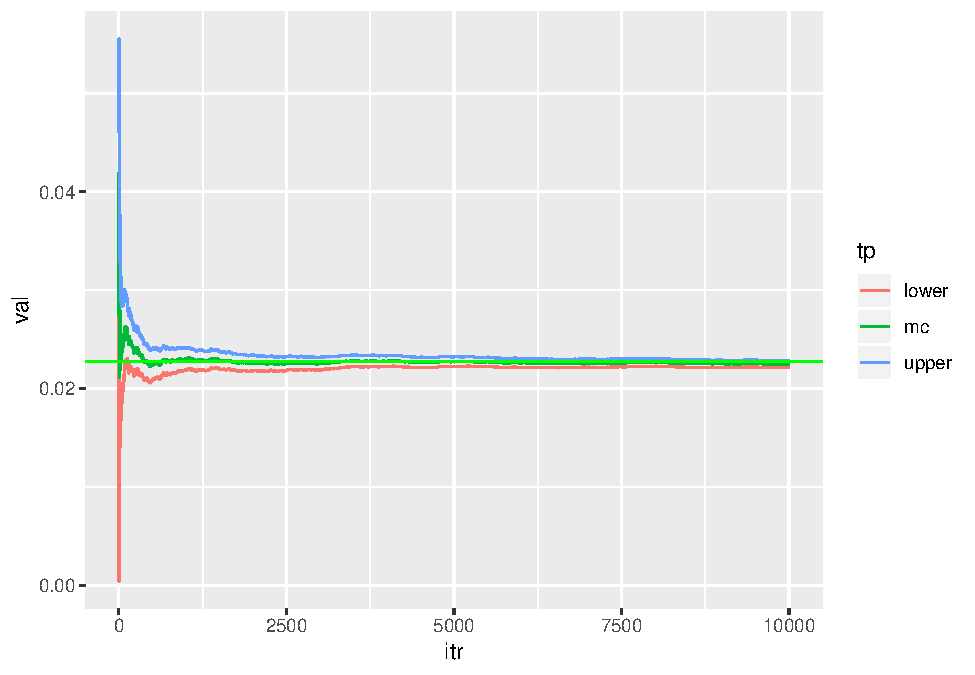
\includegraphics{bookdown-demo_files/figure-latex/unnamed-chunk-22-1.pdf}

\begin{Shaded}
\begin{Highlighting}[]
\KeywordTok{plot}\NormalTok{(fit_C}\OperatorTok{$}\NormalTok{theta[,}\DecValTok{2}\NormalTok{],}\DataTypeTok{main=}\StringTok{"Estimated Ideology Scores (Conservative Users)"}\NormalTok{,}
     \DataTypeTok{xlab=}\StringTok{"Iteration Process"}\NormalTok{,}\DataTypeTok{ylab=}\StringTok{"Ideology Scores"}\NormalTok{,}\DataTypeTok{type=}\StringTok{"l"}\NormalTok{)}
\end{Highlighting}
\end{Shaded}

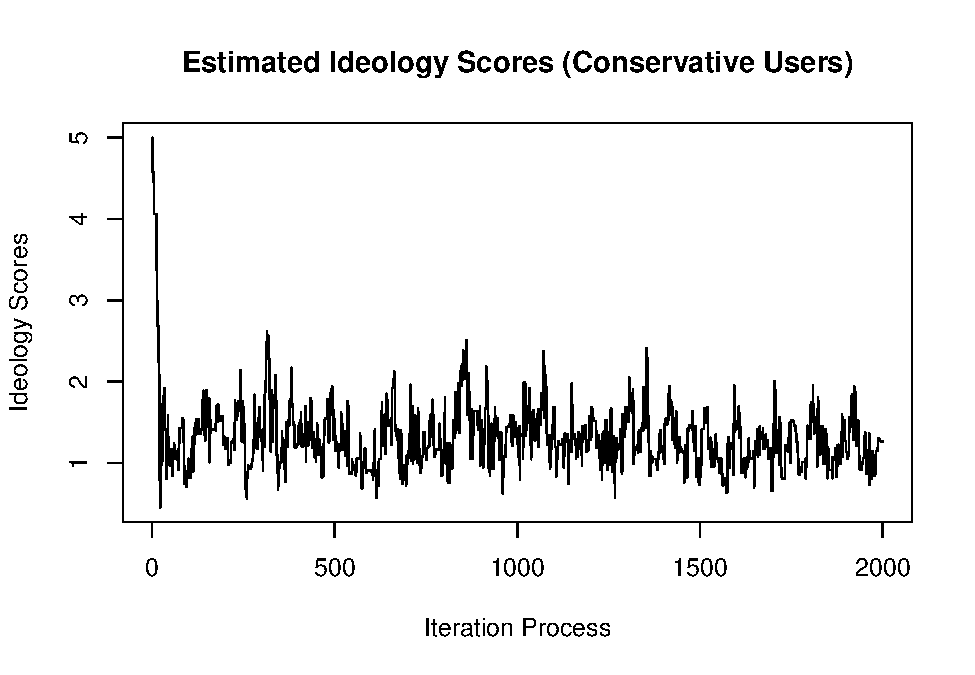
\includegraphics{bookdown-demo_files/figure-latex/unnamed-chunk-22-2.pdf}

\begin{Shaded}
\begin{Highlighting}[]
\KeywordTok{hist}\NormalTok{(fit_C}\OperatorTok{$}\NormalTok{theta[,}\DecValTok{2}\NormalTok{],}\DataTypeTok{main=}\StringTok{"Estimated Ideology Scores (Conservative Users)"}\NormalTok{,}
     \DataTypeTok{xlab=}\StringTok{"Ideology Scores"}\NormalTok{,}\DataTypeTok{breaks =} \DecValTok{100}\NormalTok{)}
\end{Highlighting}
\end{Shaded}

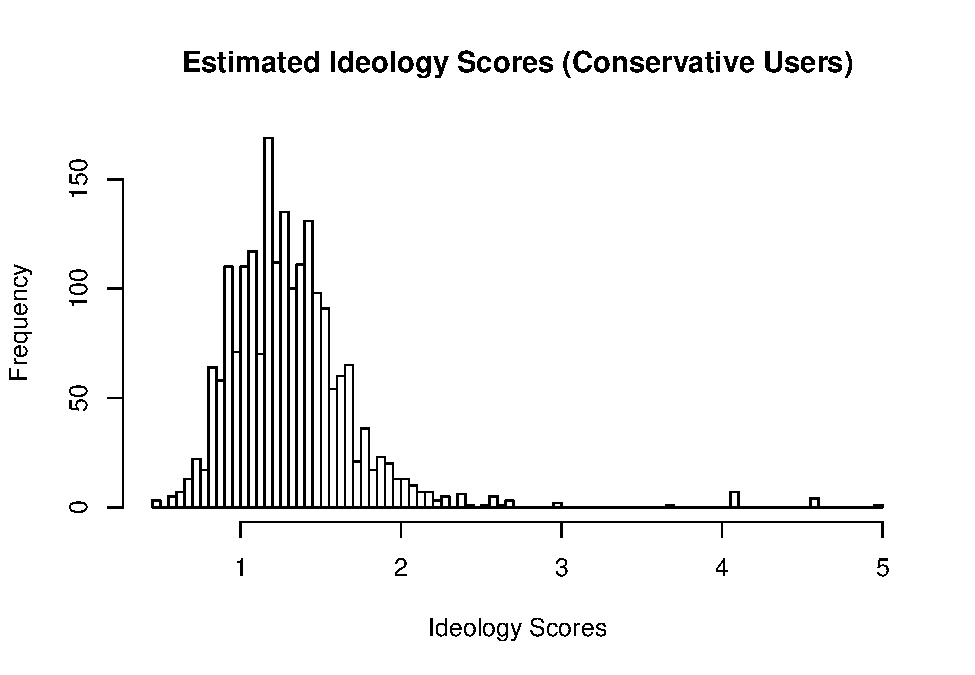
\includegraphics{bookdown-demo_files/figure-latex/unnamed-chunk-22-3.pdf}

\section{Simulating Data of Liberal Users on Twitter and Model
Testing}\label{simulating-data-of-liberal-users-on-twitter-and-model-testing}

To further verify the Metropolis Hastings algorithm, I plan to test the
opposite estimate. Specifically, assume that we observe another user,
who is more liberal. To simulate Twitter following data for this user, I
assign this user to follow more Democrat senators. In this case, we
would expect to see a negative value for their estimated ideology. As we
can see in the histogram shown below, as expected, the estimated value
is negative, providing convergent evidence for the model and the
algorithm.

\begin{Shaded}
\begin{Highlighting}[]
\CommentTok{#This user approximately follows 10 Republican Senators and 45 Democrat Senators. }
\NormalTok{Data_user<-}\KeywordTok{as.data.frame}\NormalTok{(}\KeywordTok{matrix}\NormalTok{(}\KeywordTok{c}\NormalTok{(}\KeywordTok{ifelse}\NormalTok{(}\KeywordTok{runif}\NormalTok{(}\DecValTok{50}\NormalTok{)}\OperatorTok{<}\NormalTok{.}\DecValTok{8}\NormalTok{,}\DecValTok{0}\NormalTok{,}\DecValTok{1}\NormalTok{),}\KeywordTok{ifelse}\NormalTok{(}\KeywordTok{runif}\NormalTok{(}\DecValTok{50}\NormalTok{)}\OperatorTok{<}\NormalTok{.}\DecValTok{1}\NormalTok{,}\DecValTok{0}\NormalTok{,}\DecValTok{1}\NormalTok{))), }\DecValTok{100}\NormalTok{, }\DecValTok{1}\NormalTok{)}
\KeywordTok{colnames}\NormalTok{(Data_user)<-}\KeywordTok{c}\NormalTok{(}\StringTok{"L_User"}\NormalTok{)}
\NormalTok{Data_combined<-}\KeywordTok{cbind}\NormalTok{(Data_Elites,Data_user)}

\NormalTok{X_data<-Data_combined}\OperatorTok{$}\NormalTok{Elite_ideology}
\NormalTok{Y_data<-Data_combined}\OperatorTok{$}\NormalTok{L_User}


\NormalTok{fit_L<-}\KeywordTok{Bayes_logit}\NormalTok{(Y_data,X_data)}
\NormalTok{fit_L}\OperatorTok{$}\NormalTok{acceptance_rate}
\end{Highlighting}
\end{Shaded}

\begin{verbatim}
## [1] 0.2081041 0.4337169
\end{verbatim}

\begin{Shaded}
\begin{Highlighting}[]
\KeywordTok{plot}\NormalTok{(fit_L}\OperatorTok{$}\NormalTok{theta[,}\DecValTok{1}\NormalTok{],}\DataTypeTok{main=}\StringTok{"Constant (Liberal Users)"}\NormalTok{,}
     \DataTypeTok{xlab=}\StringTok{"Iteration Process"}\NormalTok{,}\DataTypeTok{ylab=}\StringTok{"Estimated Scores"}\NormalTok{,}\DataTypeTok{type=}\StringTok{"l"}\NormalTok{)}
\end{Highlighting}
\end{Shaded}

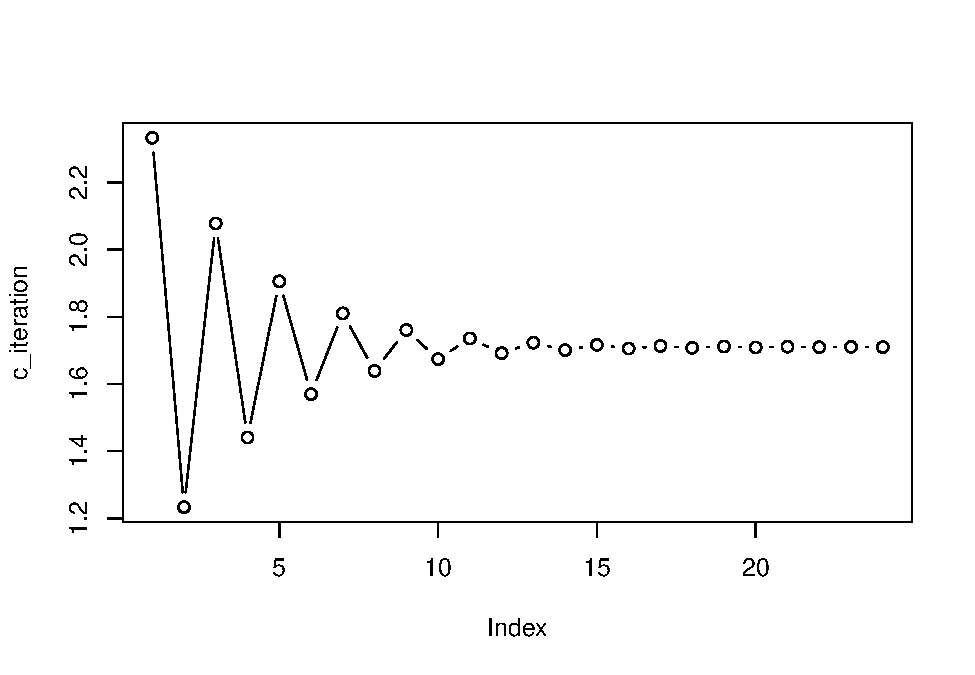
\includegraphics{bookdown-demo_files/figure-latex/unnamed-chunk-23-1.pdf}

\begin{Shaded}
\begin{Highlighting}[]
\KeywordTok{plot}\NormalTok{(fit_L}\OperatorTok{$}\NormalTok{theta[,}\DecValTok{2}\NormalTok{],}\DataTypeTok{main=}\StringTok{"Estimated Ideology Scores (Liberal Users)"}\NormalTok{,}
     \DataTypeTok{xlab=}\StringTok{"Iteration Process"}\NormalTok{,}\DataTypeTok{ylab=}\StringTok{"Ideology Scores"}\NormalTok{,}\DataTypeTok{type=}\StringTok{"l"}\NormalTok{)}
\end{Highlighting}
\end{Shaded}

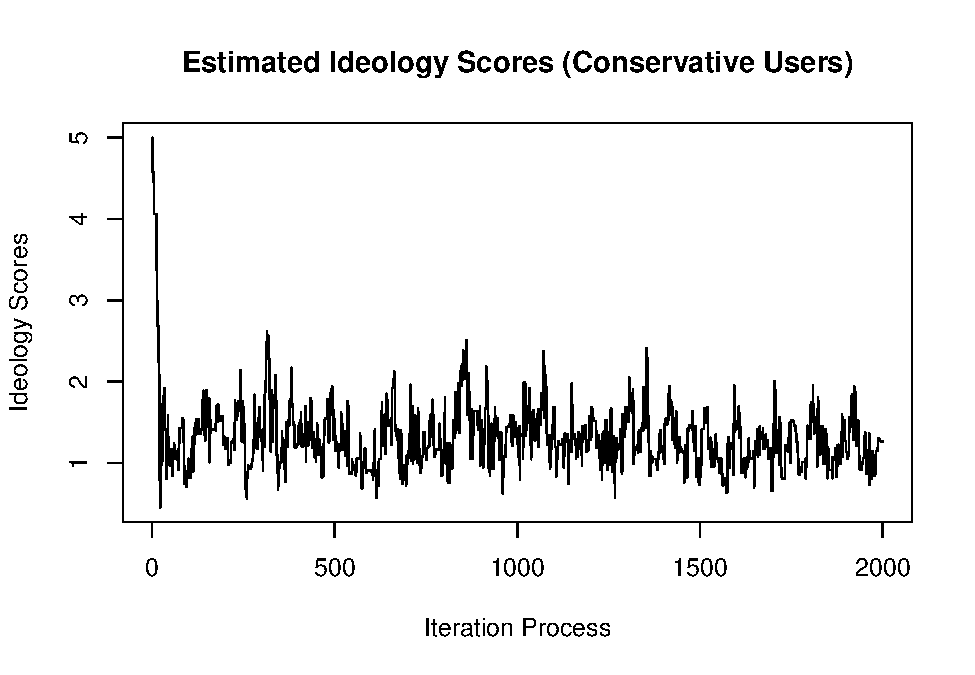
\includegraphics{bookdown-demo_files/figure-latex/unnamed-chunk-23-2.pdf}

\begin{Shaded}
\begin{Highlighting}[]
\KeywordTok{hist}\NormalTok{(fit_L}\OperatorTok{$}\NormalTok{theta[,}\DecValTok{2}\NormalTok{],}\DataTypeTok{main=}\StringTok{"Estimated Ideology Scores (Liberal Users)"}\NormalTok{,}
     \DataTypeTok{xlab=}\StringTok{"Ideology Scores"}\NormalTok{,}\DataTypeTok{breaks =} \DecValTok{100}\NormalTok{)}
\end{Highlighting}
\end{Shaded}

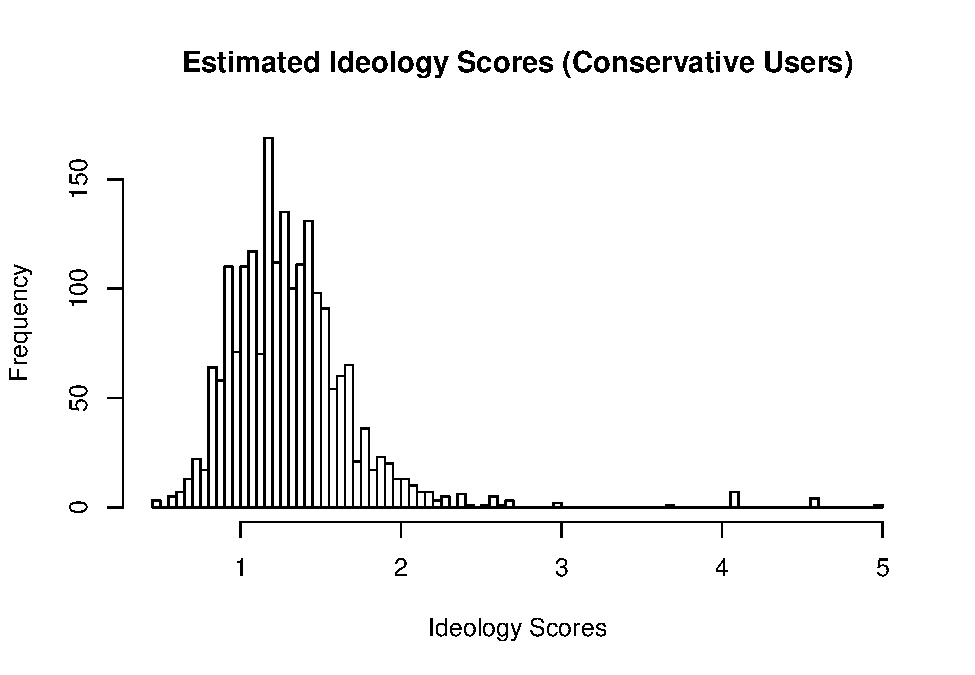
\includegraphics{bookdown-demo_files/figure-latex/unnamed-chunk-23-3.pdf}

\bibliography{book.bib,packages.bib}

\end{document}
